As already discussed in the previous section, in order to get an insight into the dynamics of the system it is interesting to consider a single uncoupled oscillator in \cref{eq:identical_diffusively}
with $m=2$. The dynamics of the system follows:
\begin{equation}
\begin{aligned}
    \tau_m \dot{s}_{11}&=-s_{11}-a_{11}+ k o_{11} \\
    \tau_a \dot{a}_{11}&=g_a o_{11} - a_{11} \\
    \tau_m \dot{s}_{12}&=-s_{12}-a_{12}+ k o_{12} \\
    \tau_a \dot{a}_{12}&=g_a o_{12} - a_{12} \\
\end{aligned}
\label{eq:complete_dynamics}
\end{equation}

The system described in \eqref{eq:complete_dynamics} is a 4 dimensional system but its analysis can be easily simplified by exploiting some nice properties of the output softmax function. In particular the two following properties hold:  
\begin{equation}
 \sum_{k=1}^{N} o_{i k}=1
 \label{soft_sum}
\end{equation}
\begin{equation}
 f(d_i)= o_{i1}-o_{i2}=\frac{e^{d_i}-1}{e^{d_i}+1}, \quad d_i = s_{i1}-s_{i2}
 \label{soft_diff}
\end{equation}
Given \eqref{soft_sum} and \eqref{soft_diff} we can introduce the following change of variables that will help us to significantly simplify the analysis of the dynamics and also get a deeper insight into the behaviour of our system. 
\begin{equation}
\begin{aligned}
z_1 &= s_{11} + s_{12} \\
w_1 &= a_{11} + a_{12} \\
d_1 &= s_{11} - s_{12} \\
e_1 &= a_{11} - a_{12} \\
\end{aligned}
\end{equation}
The dynamics in the new coordinate follows:
\begin{equation} 
\begin{aligned}
\tau_m \dot z_1 &= - z_1 - w_1 + k\\
\tau_a \dot w_1 &= g_a - w_1
\end{aligned}
\label{eq:sum_dynamics}
\end{equation}
\begin{equation} 
\begin{aligned}
\tau_m \dot d_{1} &= - d_1 - e_1 + k f(d_1) \\
\tau_a \dot{e}_{1} &= g_a f(d_1) - e_{1} \\
\end{aligned}
\label{eq:diff_dynamics}
\end{equation}

The dynamics of coupled variables $(z_1, w_1)$ is linear and it trivially holds that the equilibrium point $(z_1^*,w_1^*)=(-g_a+k, g_a)$ is globally asymptotically stable. Furthermore, it is interesting to notice that the variables  $(z_1, w_1)$ are completely decoupled from $(d_1, e_1)$. The nonlinear dynamics of the former is much richer and requires further analysis. 

\paragraph{Bifurcation Analysis}
We start the analysis of the two dimensional system in \cref{eq:diff_dynamics} by computing the equilibria $(d_1^*,e_1^*)$ and study their stability properties with the variation of the parameters $k, g_a$. As discussed in \cite{LansnerFRC} the adaptation dynamics is much slower than the support dynamics, i.e. $\tau_a > \tau_m$. Keeping in mind that what defines the dynamics is the ratio $\tau_a/\tau_m$, for the rest of the analysis we will keep $\tau_a>1$ fixed, considered as a typical constant of the system and $\tau_m=1$. Notice that the system has a global symmetry property: for each solution $(d_1(t), e_1(t))$ it holds that also $(-d_1(t), -e_1(t))$ is a solution. The roots of the equations below \eqref{eq:eq_d_eq}, \eqref{eq:eq_e_eq} are the equilibria of the dynamics in \eqref{eq:diff_dynamics}.
\begin{equation}
 (k - g_a)f(d_1^*) - d_1^* = 0
\label{eq:eq_d_eq}
\end{equation}
\begin{equation}
e_1^* = g_a f(d_1^*)
\label{eq:eq_e_eq}
\end{equation}

The number of equilibria is uniquely defined by the quantity $k-g_a$. In particular, it is easy to show that there is a unique equilibrium for $k \leq g_a-2$, while for $k > g_a-2$ we have three equilibrium points. Unfortunately, since the equilibria can not be computed analytically we will make use of numerical analysis. In \cref{fig:eq2D_adapt} the three most important cases are plotted.

 \begin{figure}[!h]
        \center{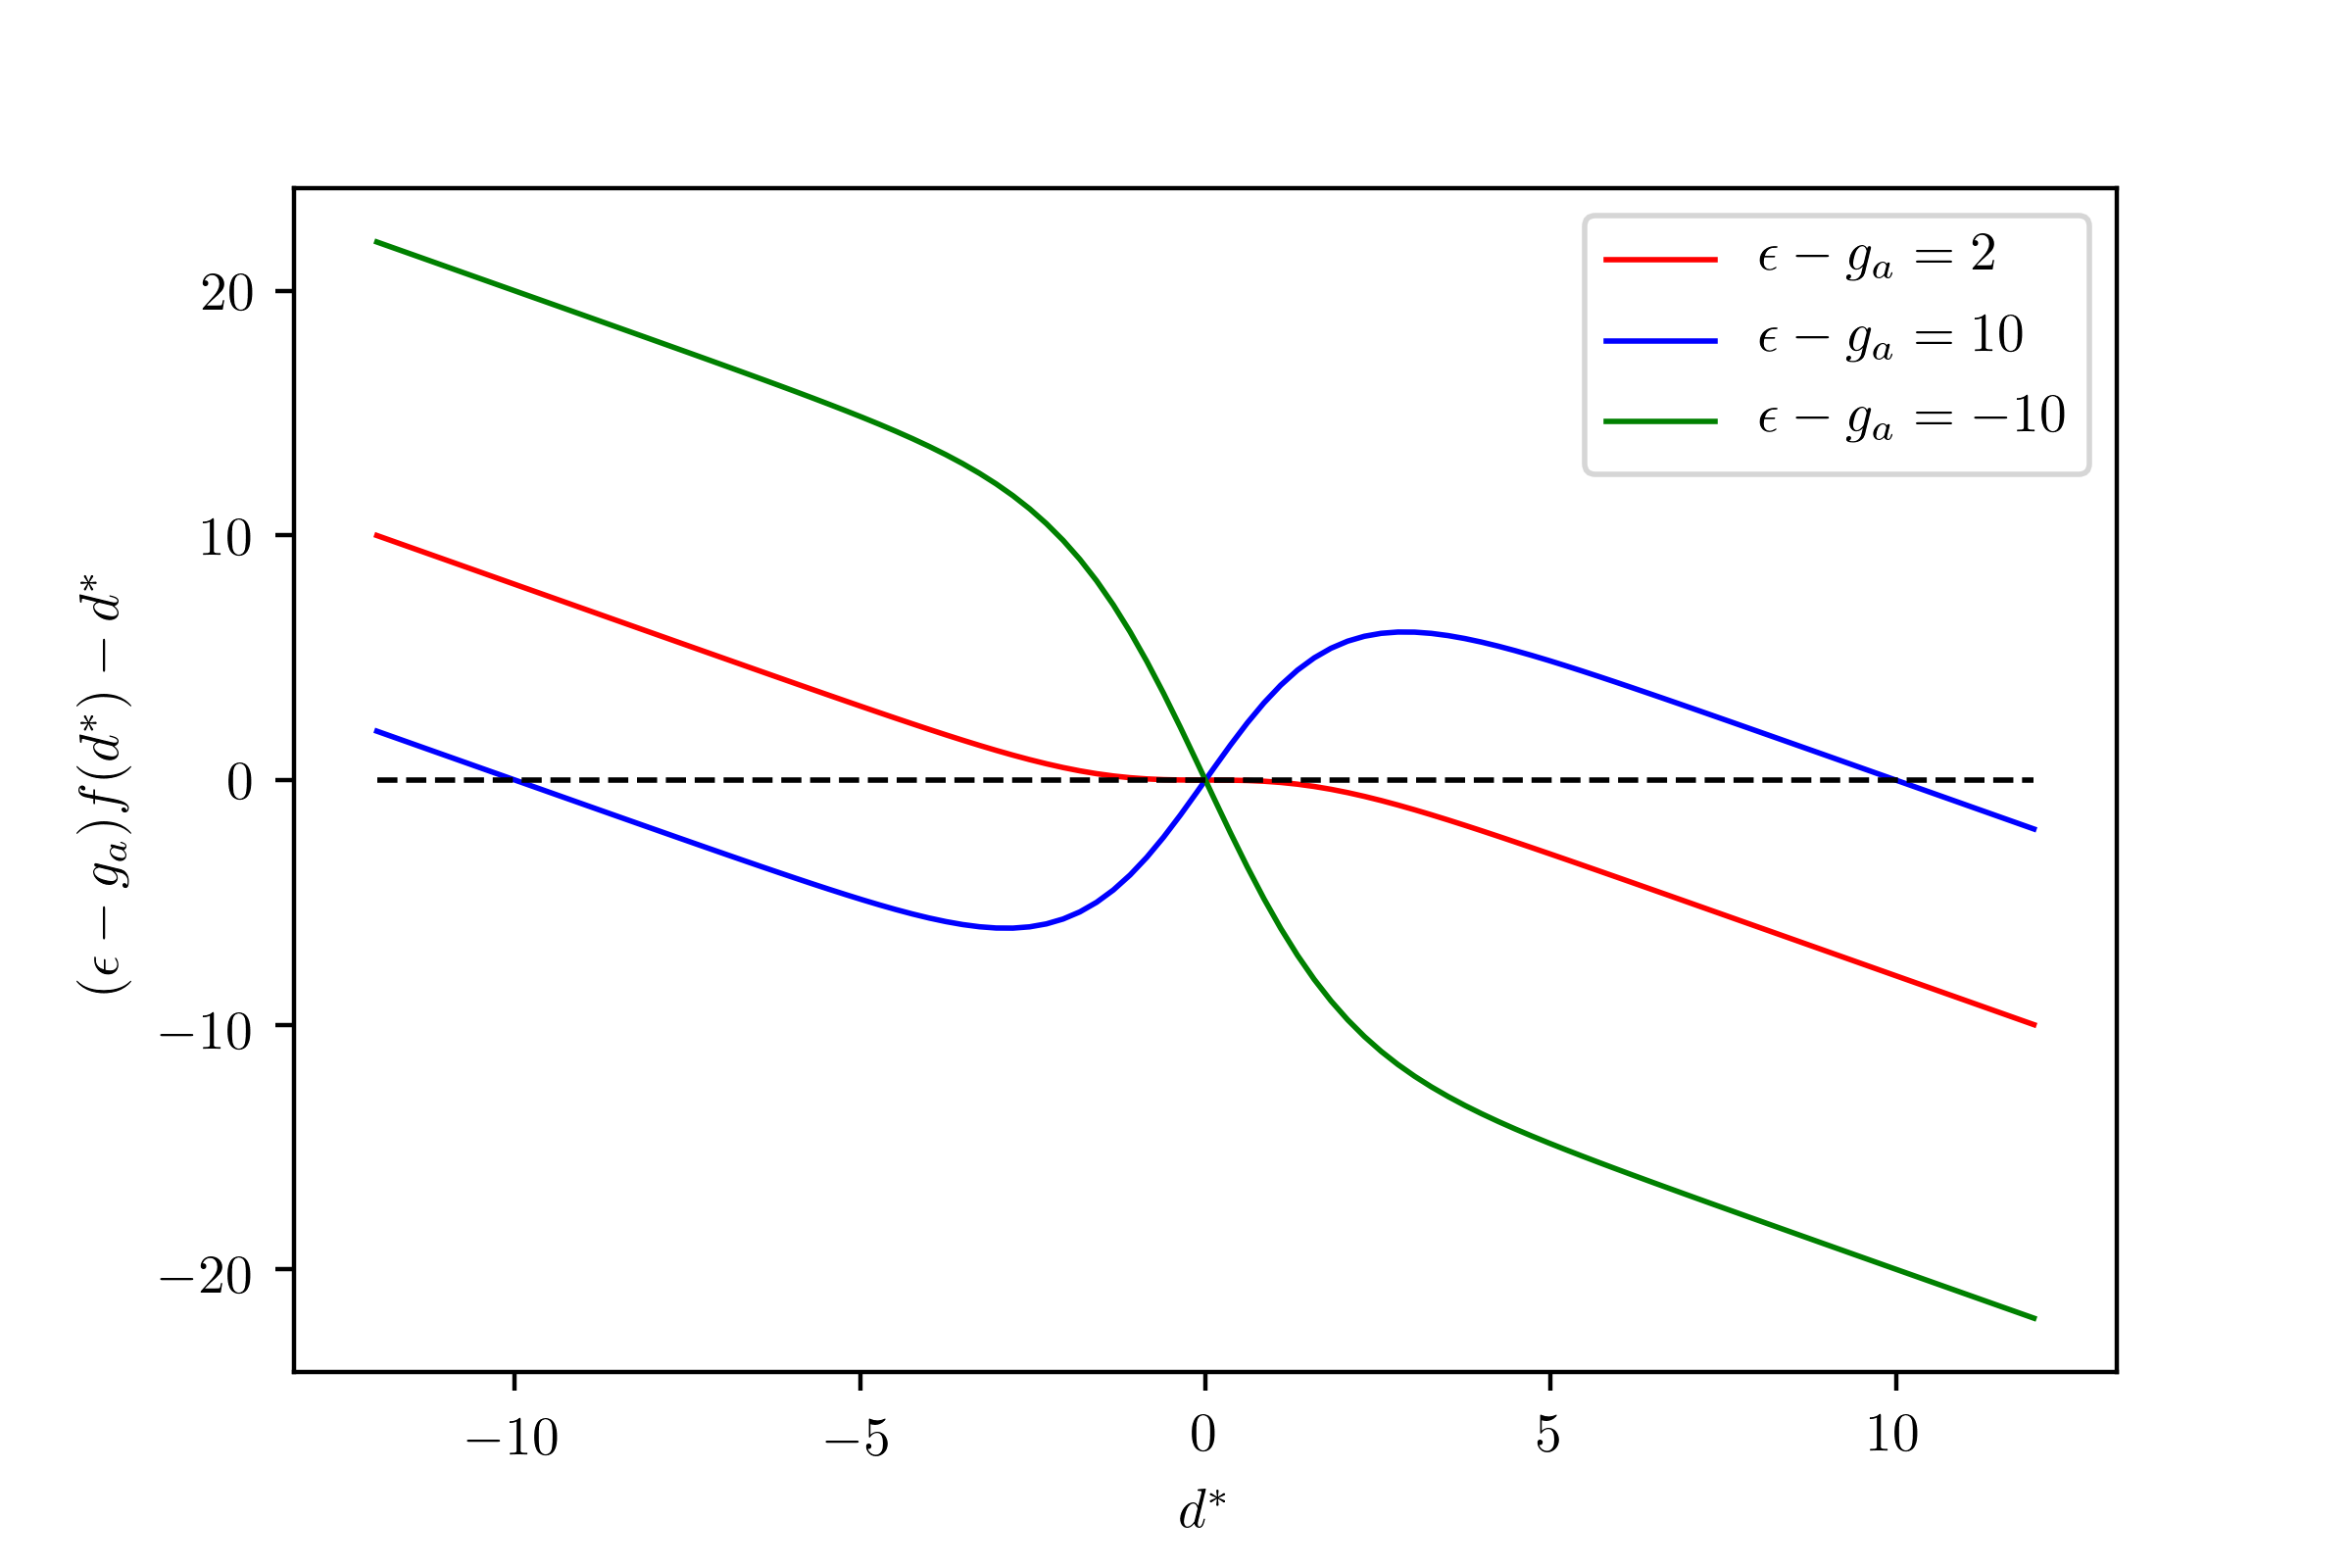
\includegraphics[width=\textwidth]{text/analysis/fig/2by2adapt/equilibria_2D.png}}
        \caption{\label{fig:eq2D_adapt} Graphical visualization of the roots of the equation in \eqref{eq:eq_d_eq}} with varying the quantity $k - g_a$.
\end{figure}

We will first analyse the system with $k - g_a < 2$. With this choice of parameters the unique equilibrium is the point $(d_1^*,e_1^*)=(0, 0)$. The computed jacobian matrix $J_{(0,0)}$ and the characteristic polynomial are the following:

\begin{equation}
J_{(0, 0)} = \begin{bmatrix} 
\frac{k}{2} & -1 \\
\frac{g_a}{2\tau_a} & -\frac{1}{\tau}
\end{bmatrix}
\end{equation}

\begin{equation}
\rho(\lambda) = \lambda^2 +  \frac{2\tau_a + 2 - \tau_a k}{2\tau_a} \lambda + \frac{-2k + 2g_a + 4}{4\tau_a}
\end{equation}

\begin{equation}
\rho(\lambda) = \lambda^2 + a\lambda +b
\end{equation}

In order to study the stability of the equilibrium point one can study the sign of the polynomial's coefficient. In fact for a second order polynomial, the number of roots with positive real part can be determined by the number of variations in the polynomial's coefficients.

\begin{equation}
\begin{aligned}
 a < 0 \iff & k > 2(1 + \frac{1}{\tau_a}) \\
 b < 0 \iff & k > g_a + 2
\end{aligned}
\end{equation}

When $k<2(1+\frac{1}{\tau_a})$ the origin is an asymptotically stable equilibrium point. This condition is not particularly interesting since it means that all the units in the network converge to the same value and their output is identical. In other words, the network is not able to recall any pattern (\cref{fig:eq2D_focus}).

\begin{figure}[H]
        \center{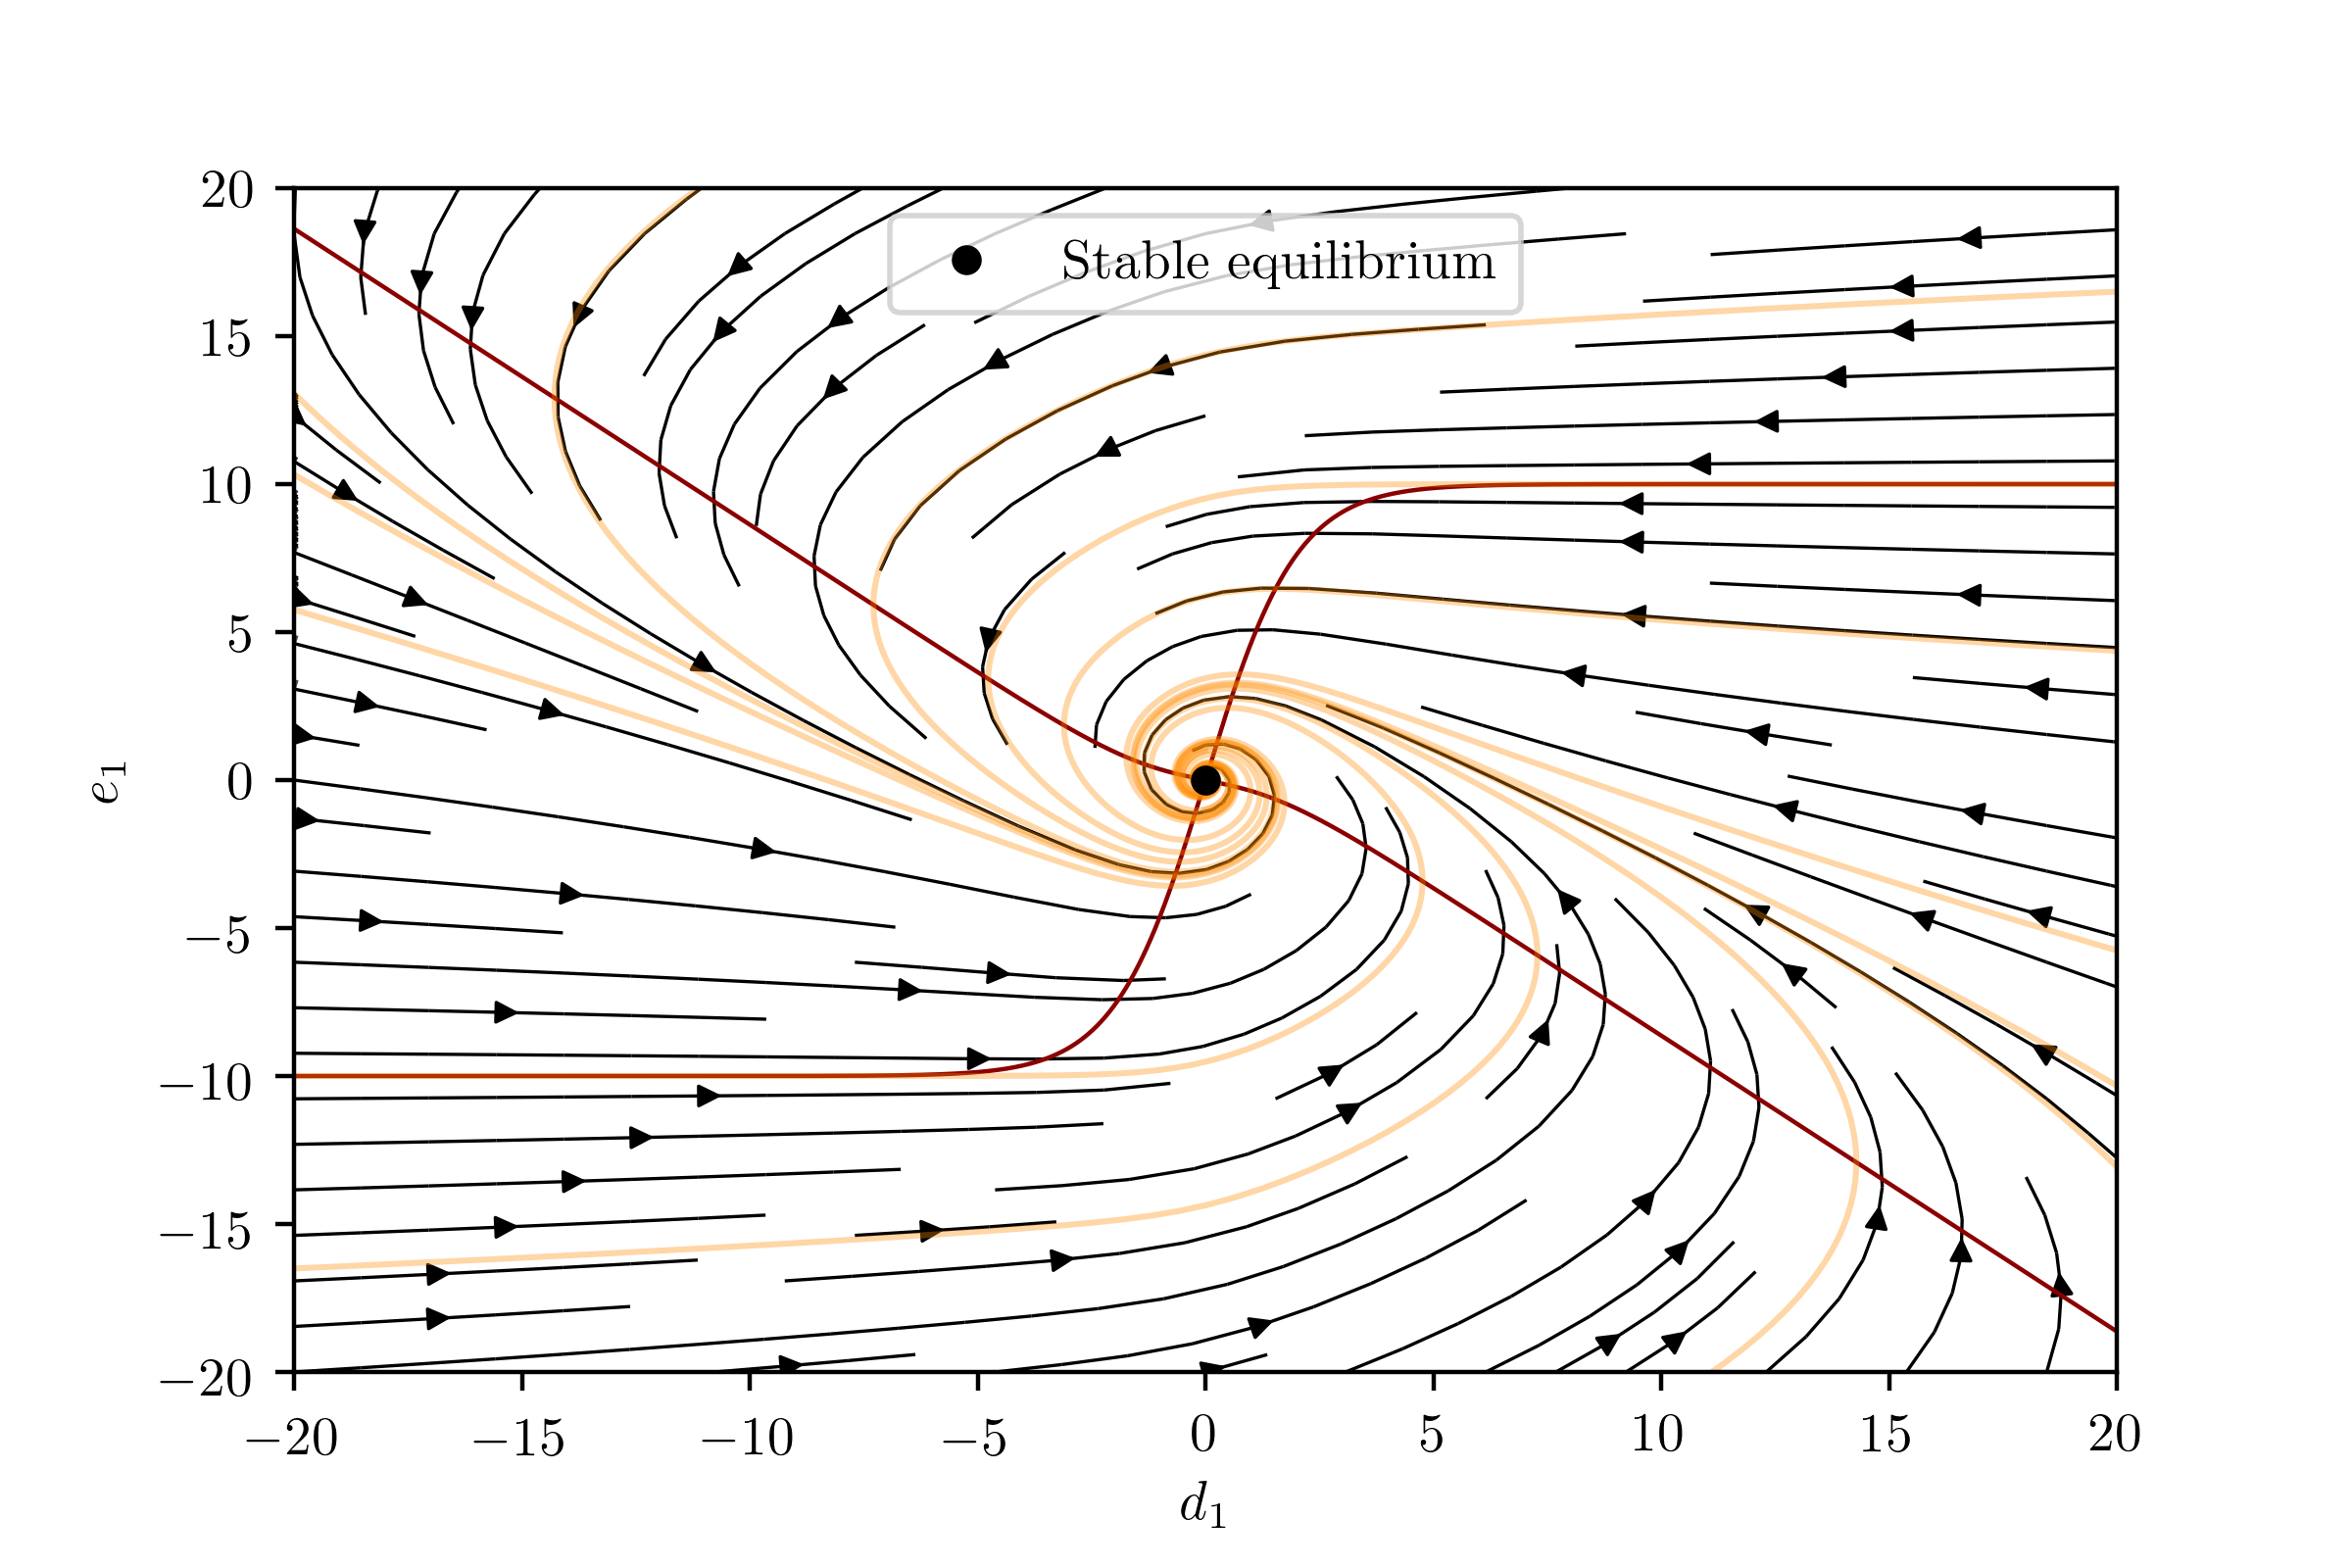
\includegraphics[width=\textwidth]{text/analysis/fig/2by2adapt/streamline_stable_focus.png}}
        \caption{\label{fig:eq2D_focus} Phase portrait of system in \eqref{eq:diff_dynamics} for $k=1.5,\ g_a=10,\ \tau_a=2$. The nullclines are shown in dark red; the streamline plot is shown in black; several trajectories of the system with different initial conditions are shown in orange.}
\end{figure}


At the critical value $k^* = 2 ( 1 + \frac{1}{\tau_a} ) $ a \textbf{supercritical Hopf} bifurcation occurs. In fact, as $k$ passes through $k^*$, the complex eigenvalues $\lambda_{1,2}$ cross the imaginary axis. In fact, ${\rm I\!R}(\lambda_{1,2})<0, k < k^*$ and  ${\rm I\!R}(\lambda_{1,2})>0, k > k^*$. Therefore, the equilibrium point $(0, 0)$ changes its stability and a unique stable limit cycle bifurcates from it (\cref{fig:eq2D_cycle}).

\begin{figure}[H]
        \center{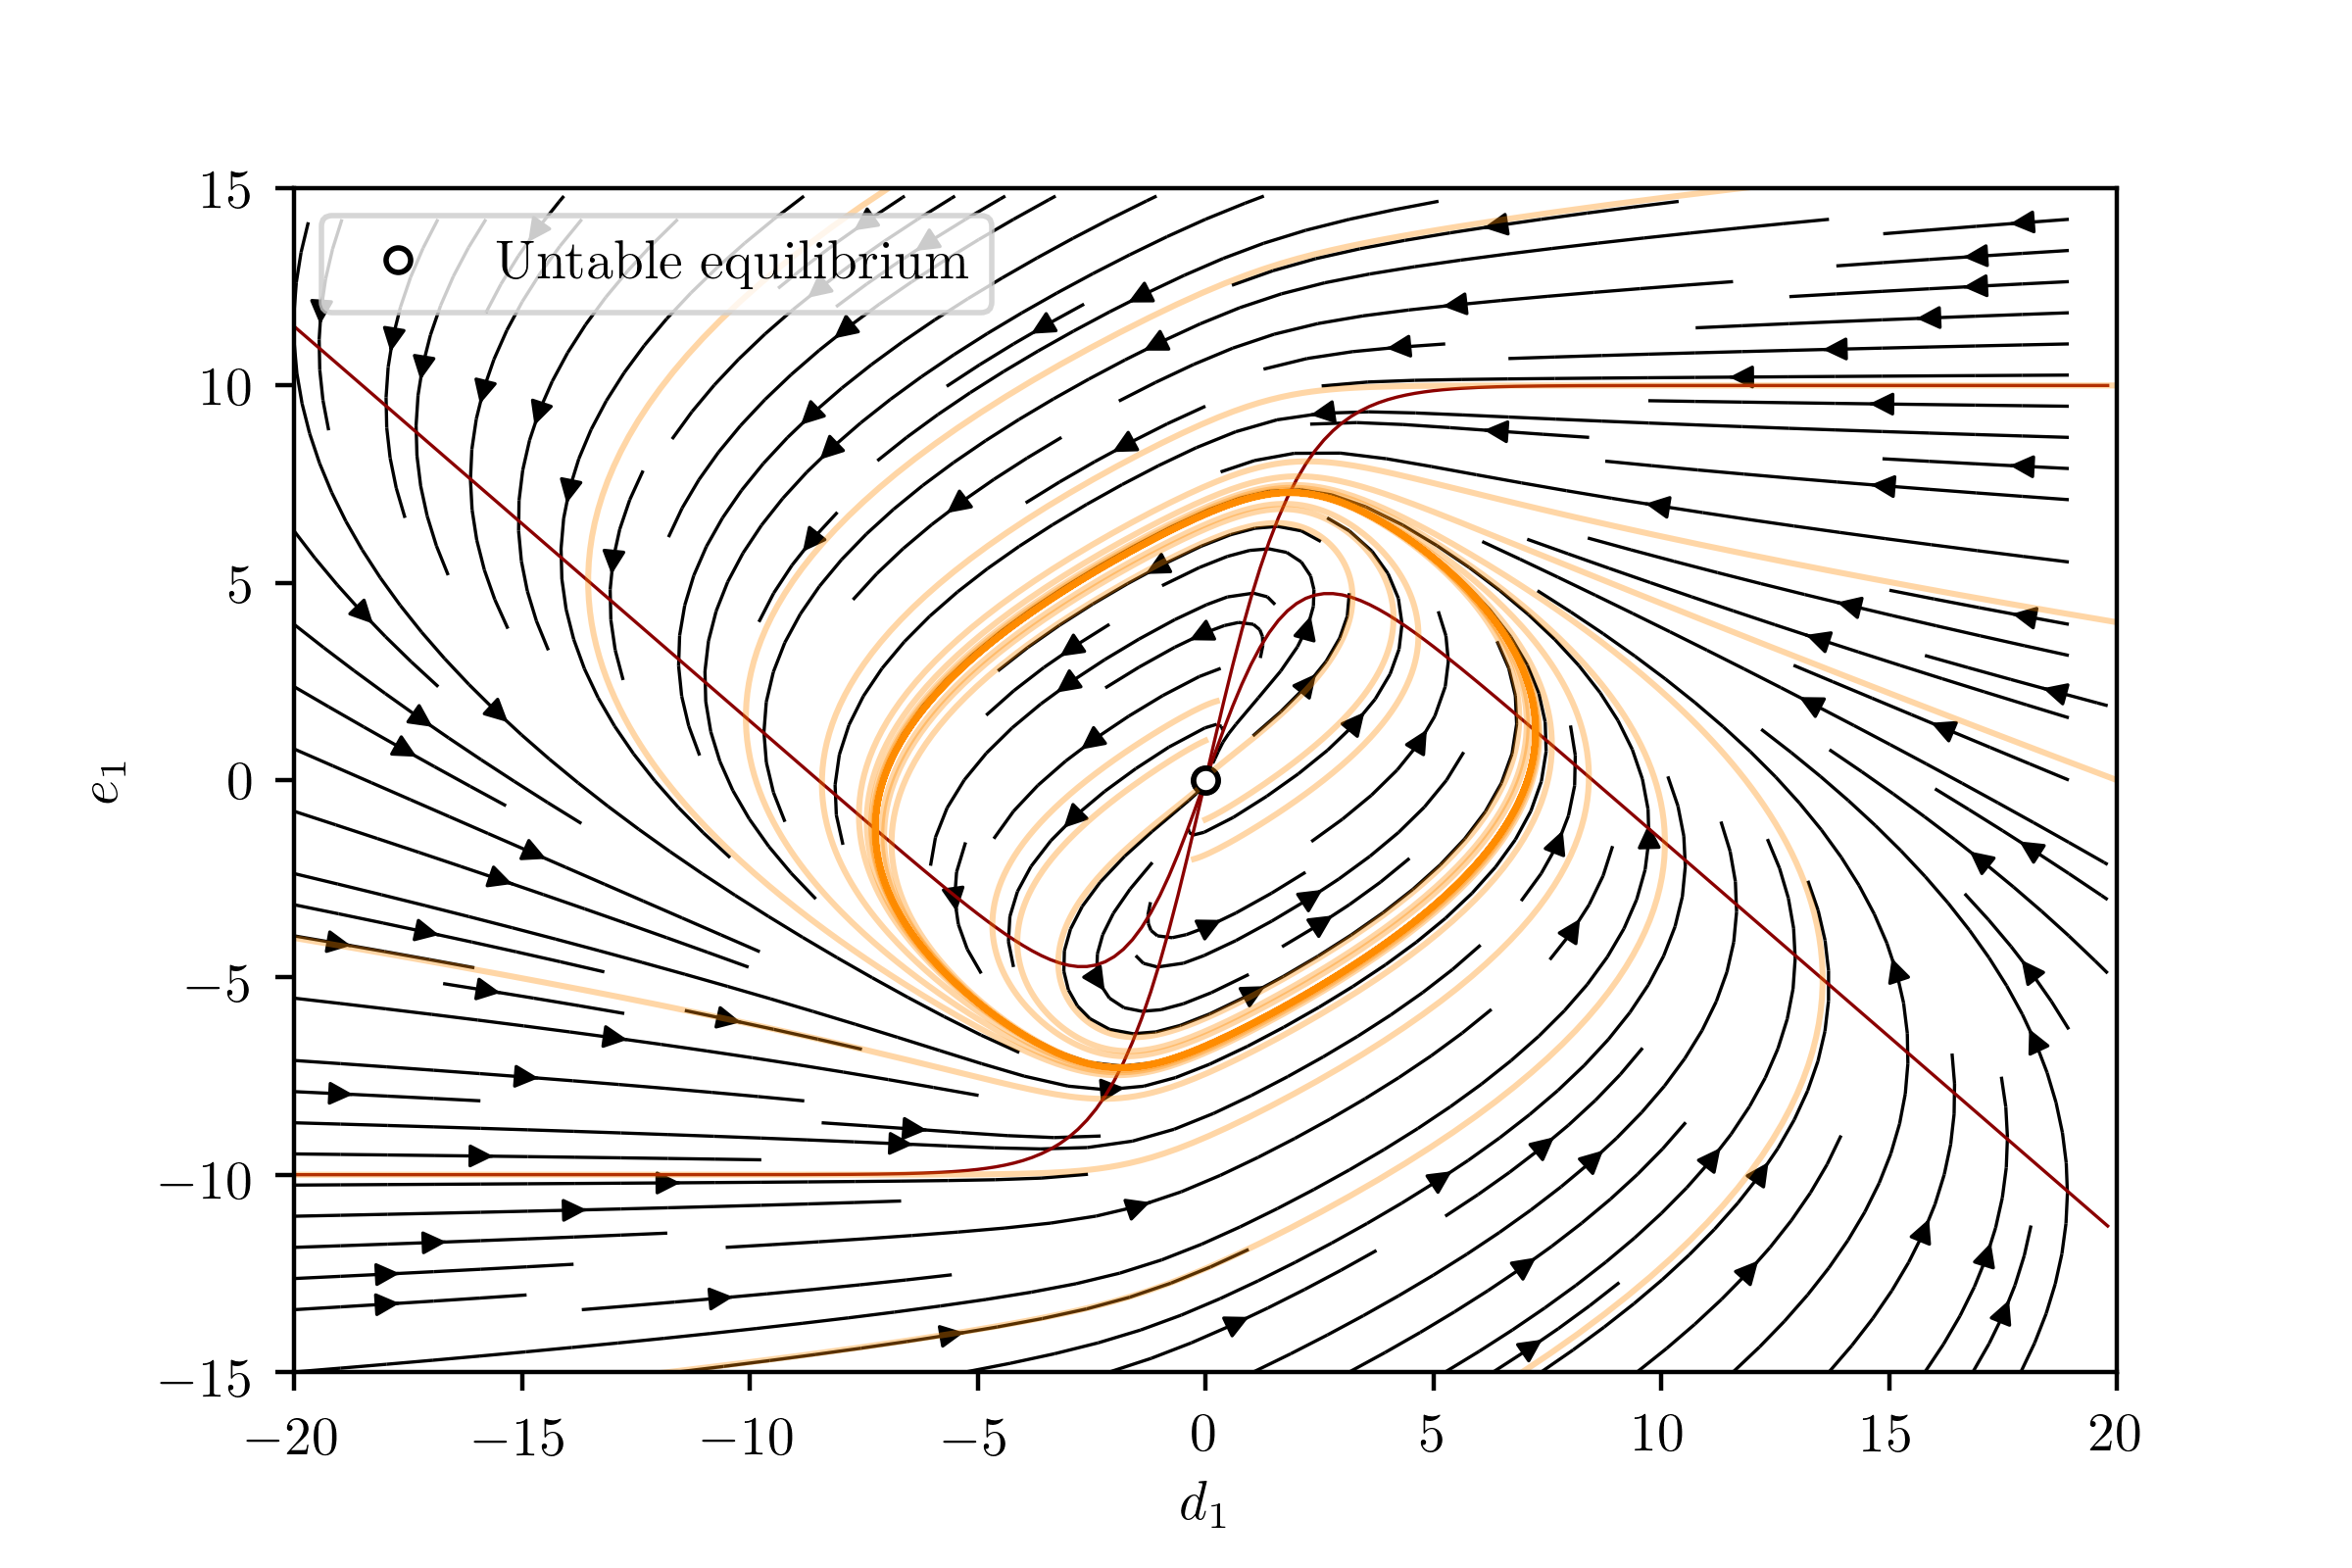
\includegraphics[width=\textwidth]{text/analysis/fig/2by2adapt/streamline_cycle.png}}
        \caption{\label{fig:eq2D_cycle} Phase portrait of system in \eqref{eq:diff_dynamics} for $k=8.5,\ g_a=10,\ \tau_a=2$. The nullclines are shown in dark red; the streamline plot is shown in black; several trajectories of the system with different initial conditions are shown in orange.}
\end{figure}

But what happens when the coupling factor $k$ increases? The next interesting bifurcation phenomenon occurs at the critical value $k^o = g_a + 2$ when a \textbf{supercritical pitchfork bifurcation} occurs. In fact, the origin spawns two unstable equilibria and changes from unstable node to saddle. While the parameter $k > k^o$ keeps increasing the additional two equilibria moves far away from the origin and additional bifurcations occur. In particular, by numerically analising the stability of the Jacbobian matrix at the two off-origin equilibria, a \textbf{subcritical Hopf bifurcation} occurs at the critical value $k^{oo} \approx 12.69$. As discussed in the preliminaries section [cite the right section], in a specular way with respect to what happens in the supercritical case, each off origin equilibria changes its stability and a unique unstable limit cycle bifurcates from each of them as shown in \cref{fig:adapt_zoom_tri_limt}. As the parameter $k$ increases the unstable limit cycles increase their size until they collide on the saddle equlibria at the origin. After this homoclinic bifurcation occurs \footnote{This is a particular type of global bifurcation that requires further analysis},
 an interesting phenomenon occurs: the two unstable limit cycles merge into a bigger limit cycle as shown in \cref{fig:eq2D_cycle_before_collapse}. The last important bifurcation consists in the mutual annihilation of the inner (unstable) and outer (stable) limit cycles after which the only attractors in the system are the two off-origin equilibria (stable) and the origin (unstable) (\cref{fig:eq2D_cycle_after_collapse}).

\iftrue
   \begin{figure*}[!h]
        \centering
        \begin{subfigure}[b]{1\textwidth}
            \centering
            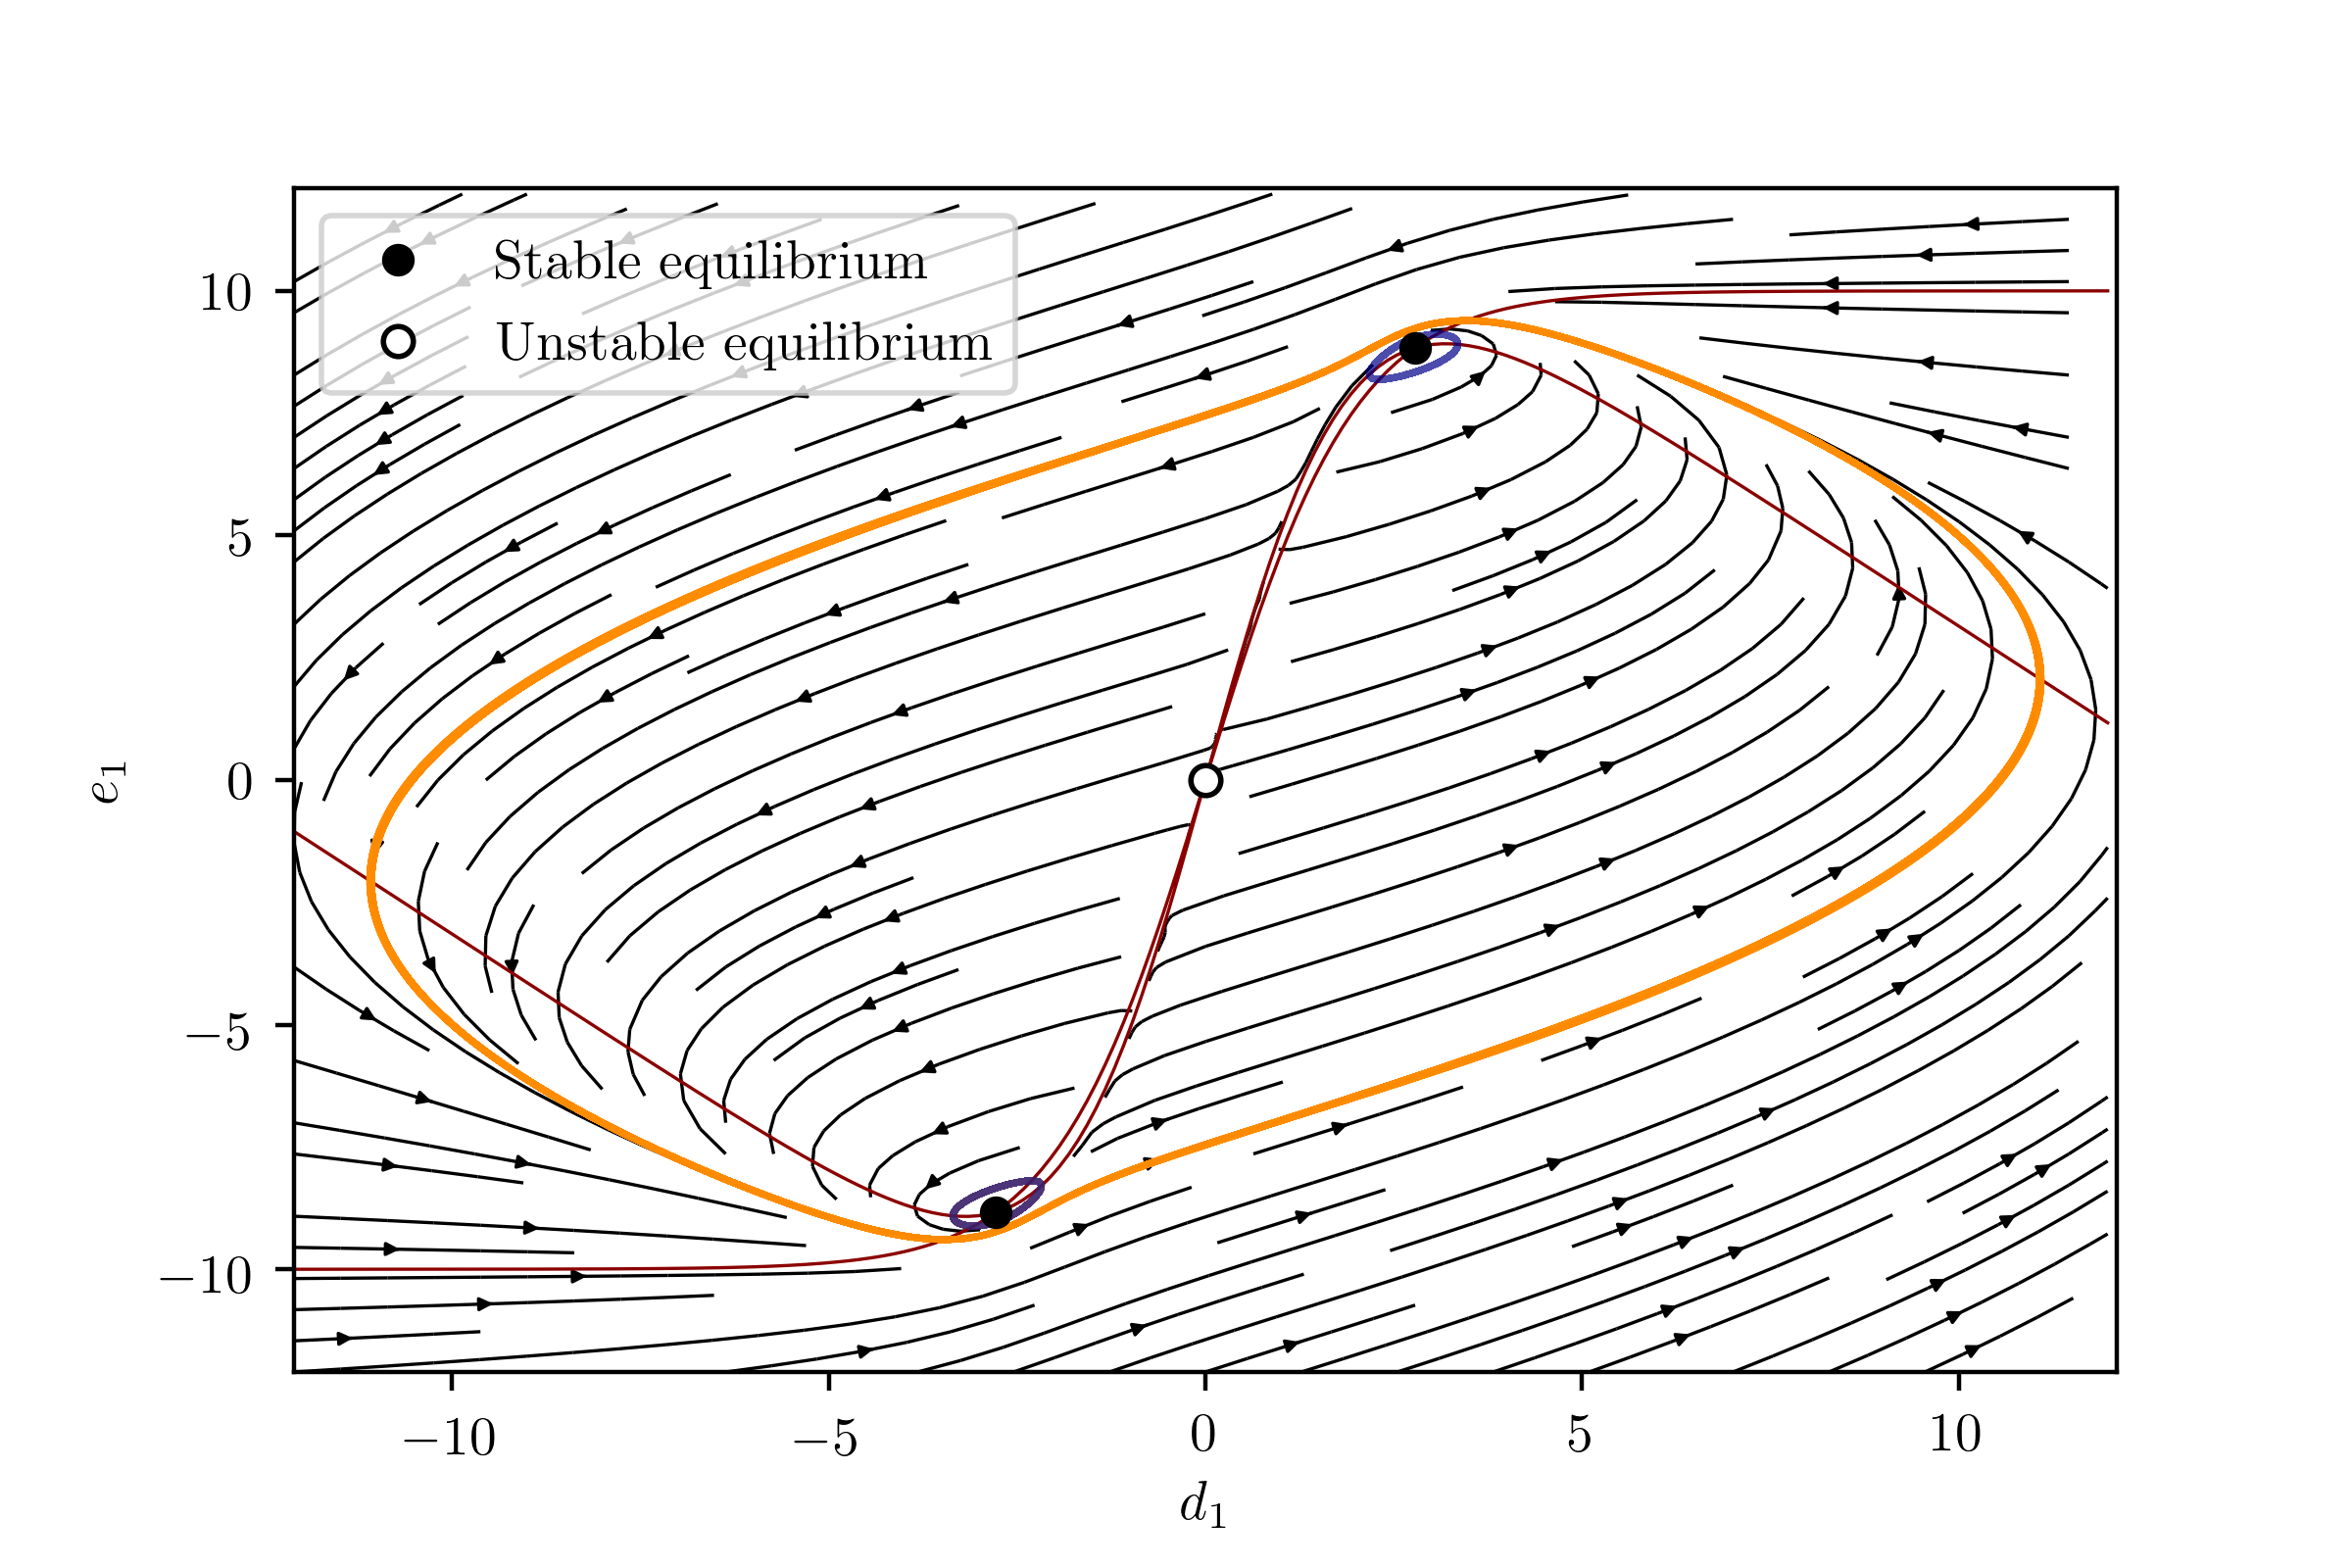
\includegraphics[width=\textwidth]{text/analysis/fig/2by2adapt/streamline_triple_limit.png}
        \end{subfigure}
        \vskip\baselineskip
        \begin{subfigure}[b]{1\textwidth}  
            \centering 
            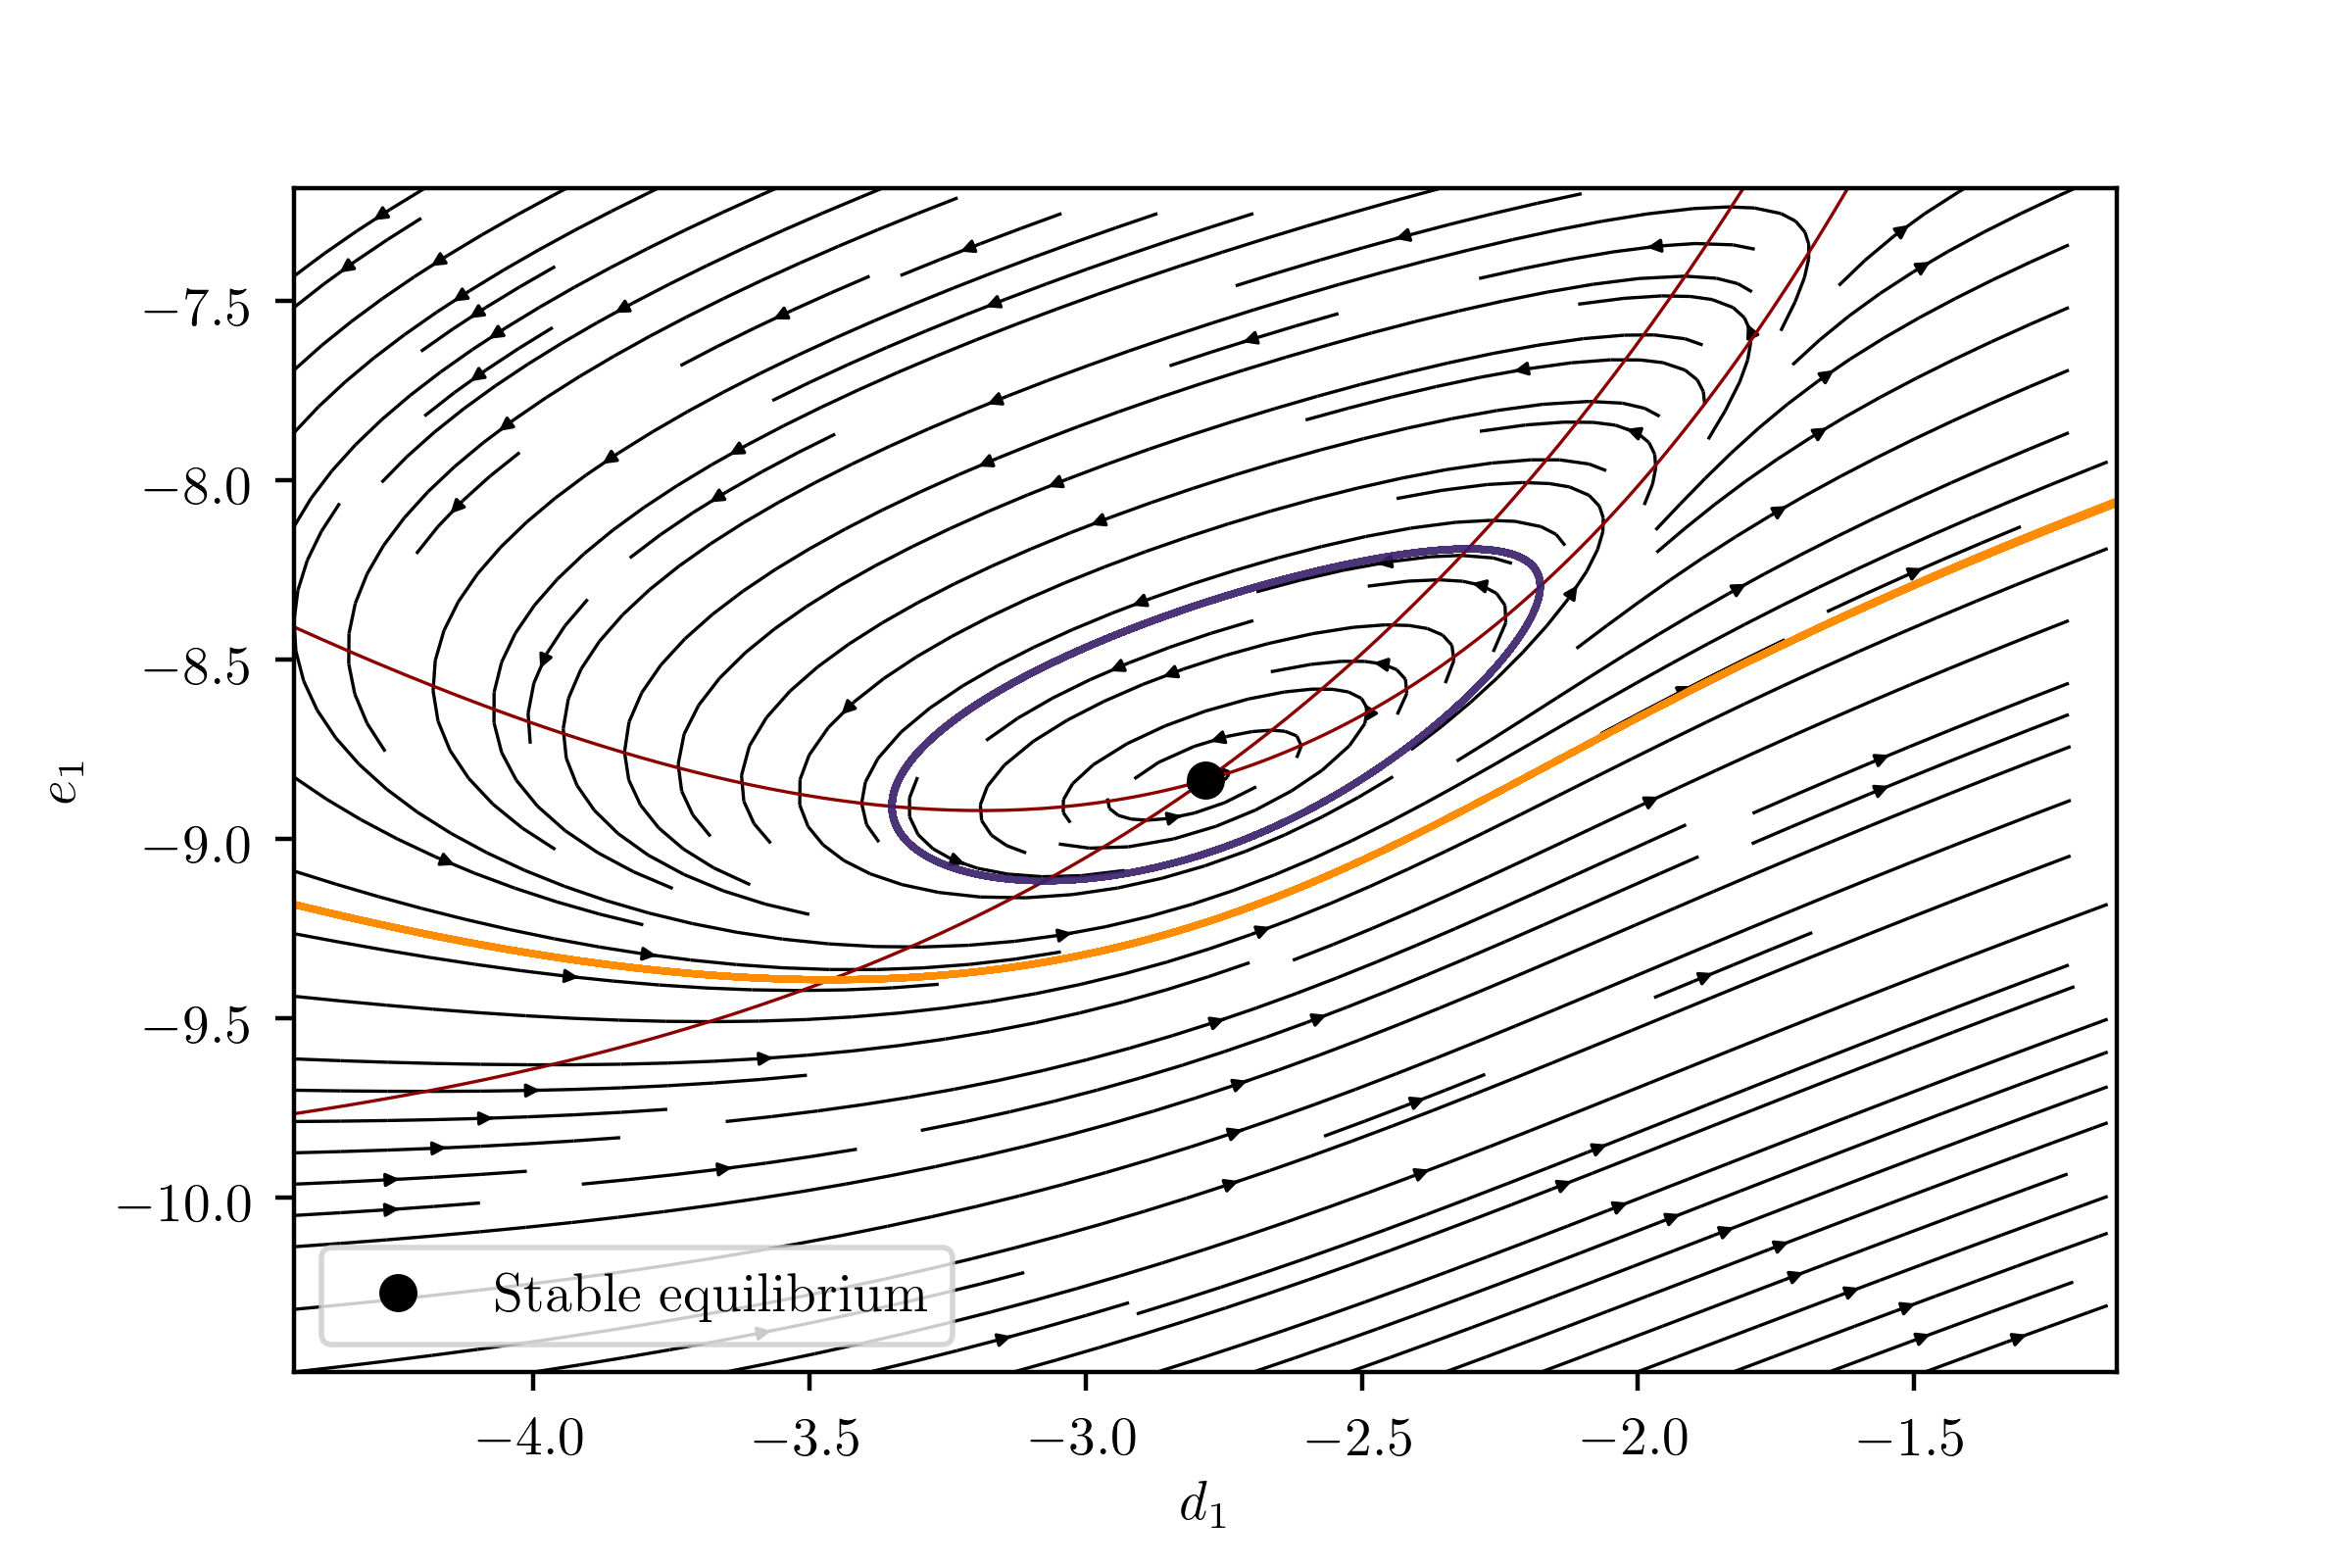
\includegraphics[width=\textwidth]{text/analysis/fig/2by2adapt/streamline_fixed_zoom.png}
        \end{subfigure}
        \caption{Phase portrait of system in \eqref{eq:diff_dynamics} for $k=13.15,\ g_a=10,\ \tau_a=2$. The nullclines are shown in dark red; the streamline plot is shown in black; the outer stable limit cycle is shown in orange; the inner unstable limit cycles (obtained by backward integration in time) are shown in blue. The two pictures show respectively the overall phase portrait (upper) and a zoom on the unstable limit cycle (lower).} 
        \label{fig:adapt_zoom_tri_limt}
    \end{figure*}
\fi


\begin{figure}[!h]
        \center{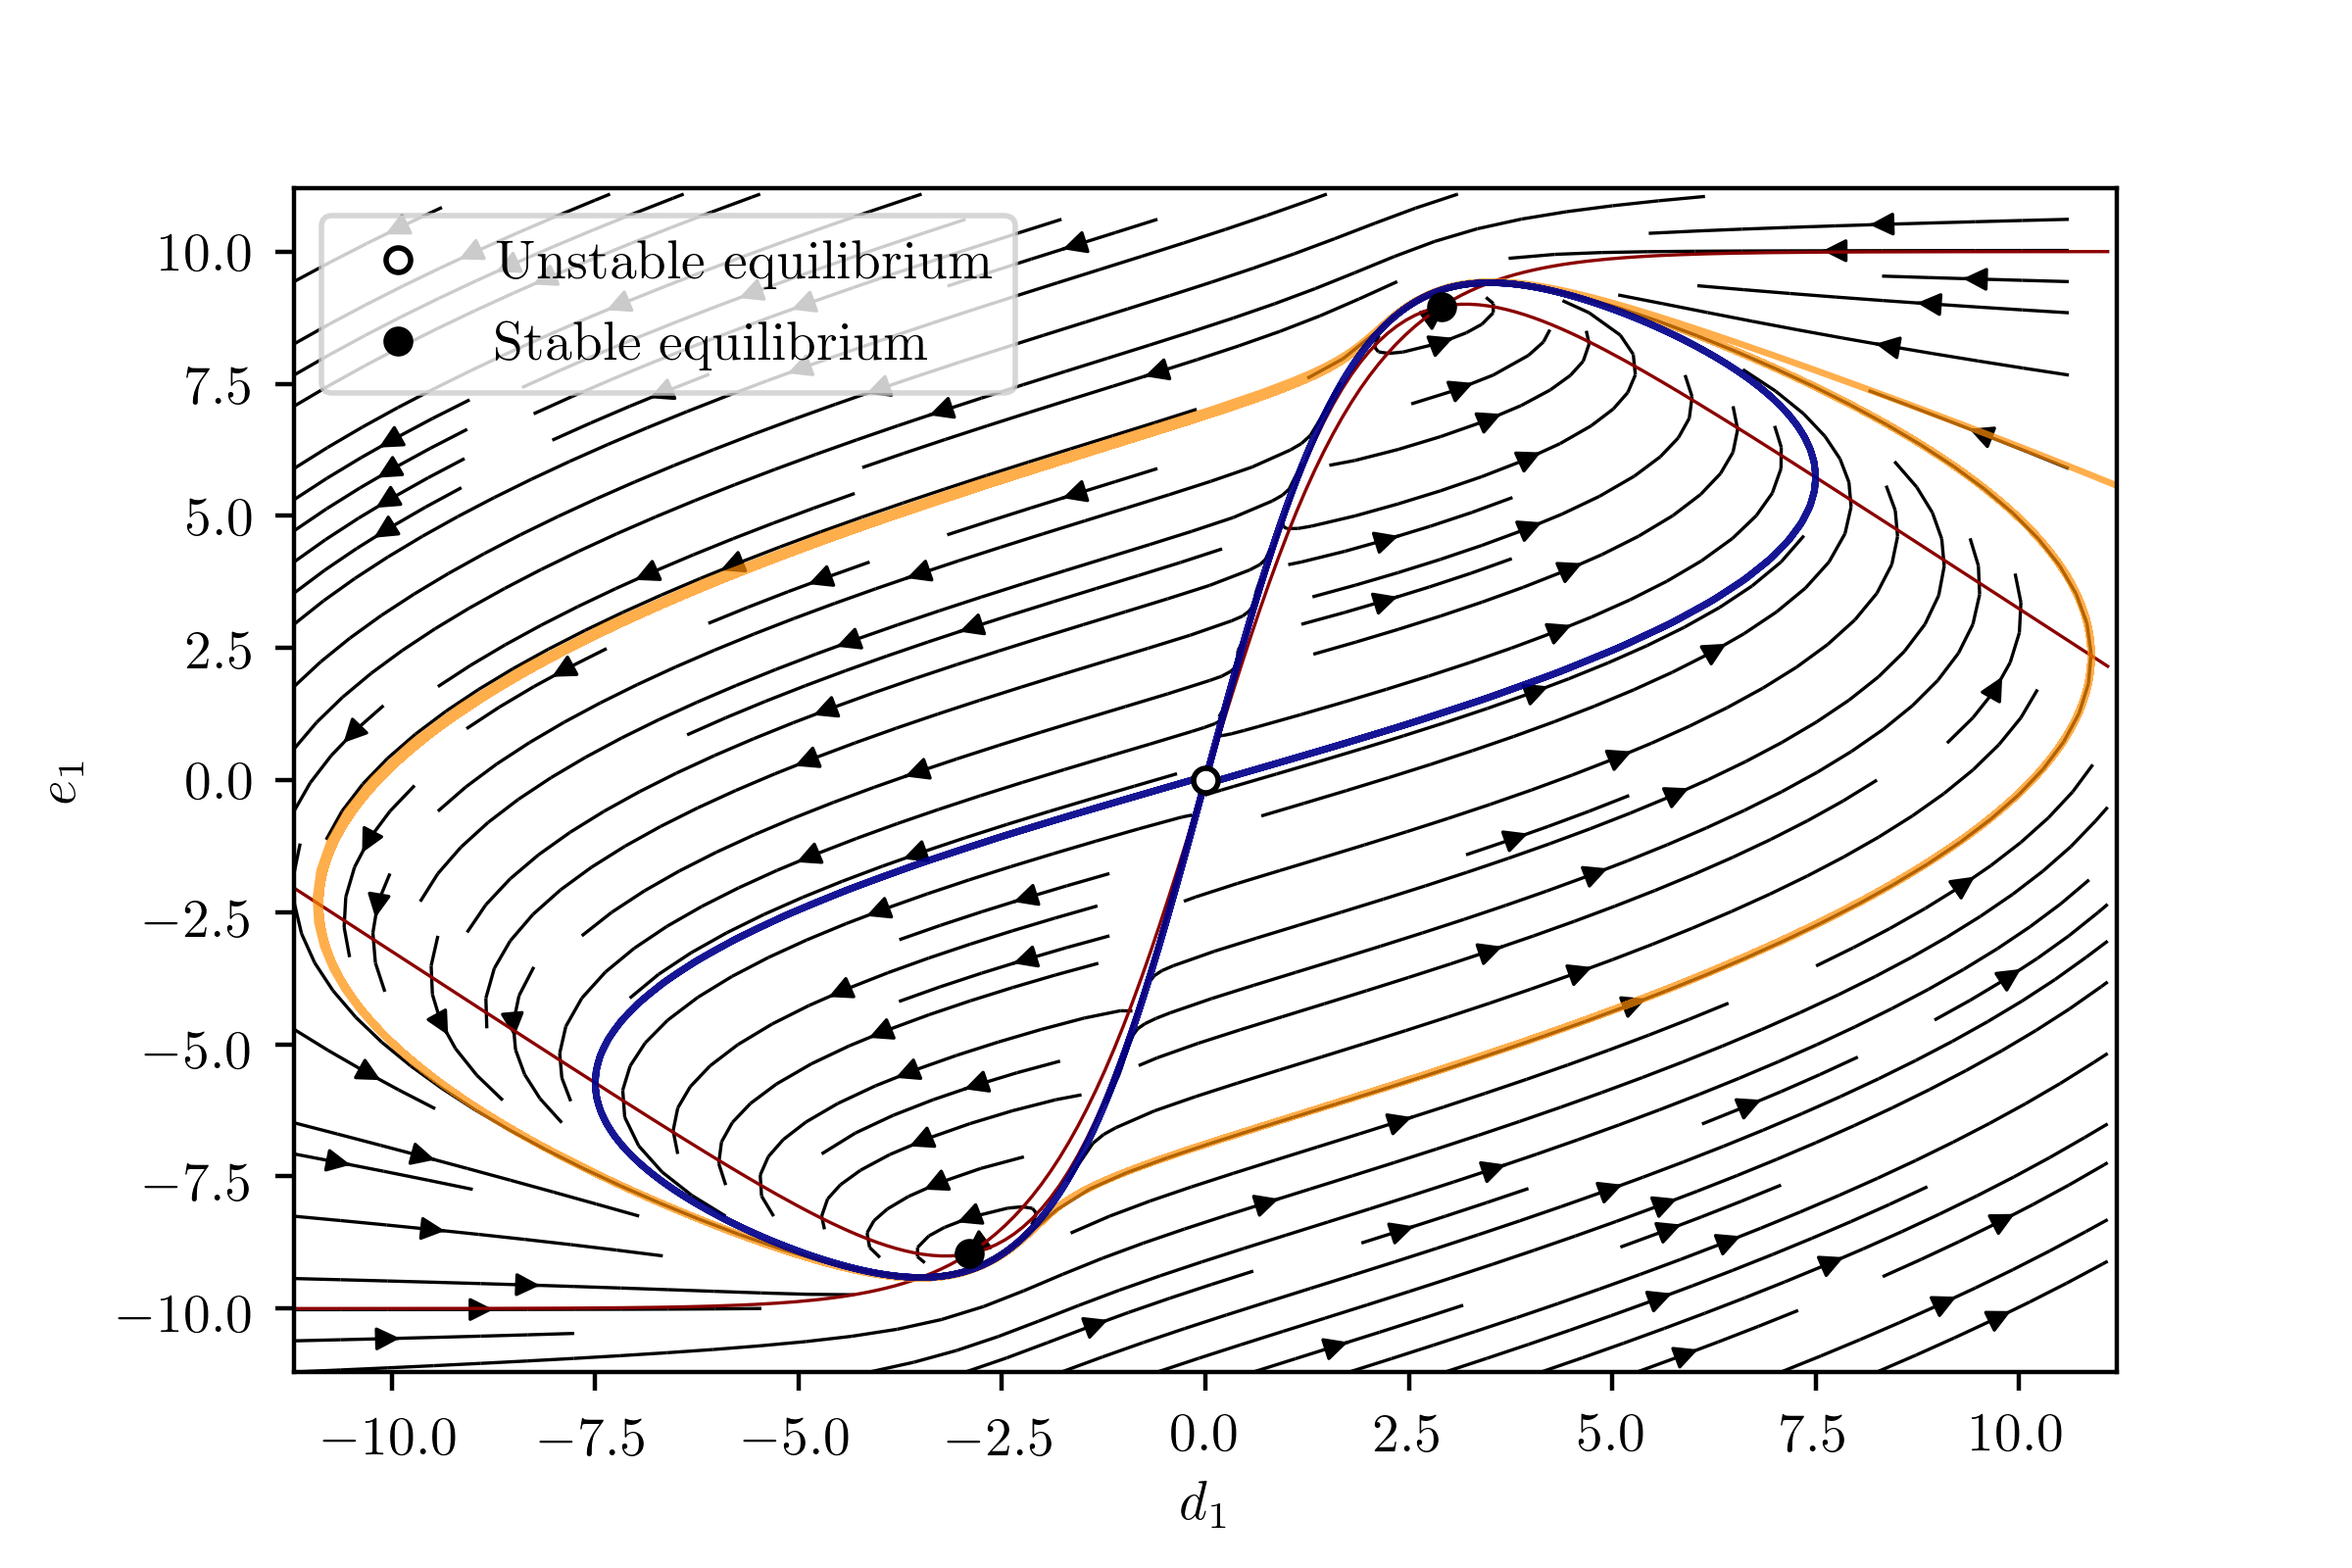
\includegraphics[width=\textwidth]{text/analysis/fig/2by2adapt/streamline_homoclinic.png}}
        \caption{\label{fig:eq2D_cycle_homoclinic} Phase portrait of system in \eqref{eq:diff_dynamics} for $k=13.2422,\ g_a=10,\ \tau_a=2$. The nullclines are shown in dark red; the streamline plot is shown in black; the outer stable limit cycle is shown in orange; the inner unstable limit cycles (obtained by backward integration in time) are shown in blue.}
\end{figure}

\begin{figure}[!h]
        \center{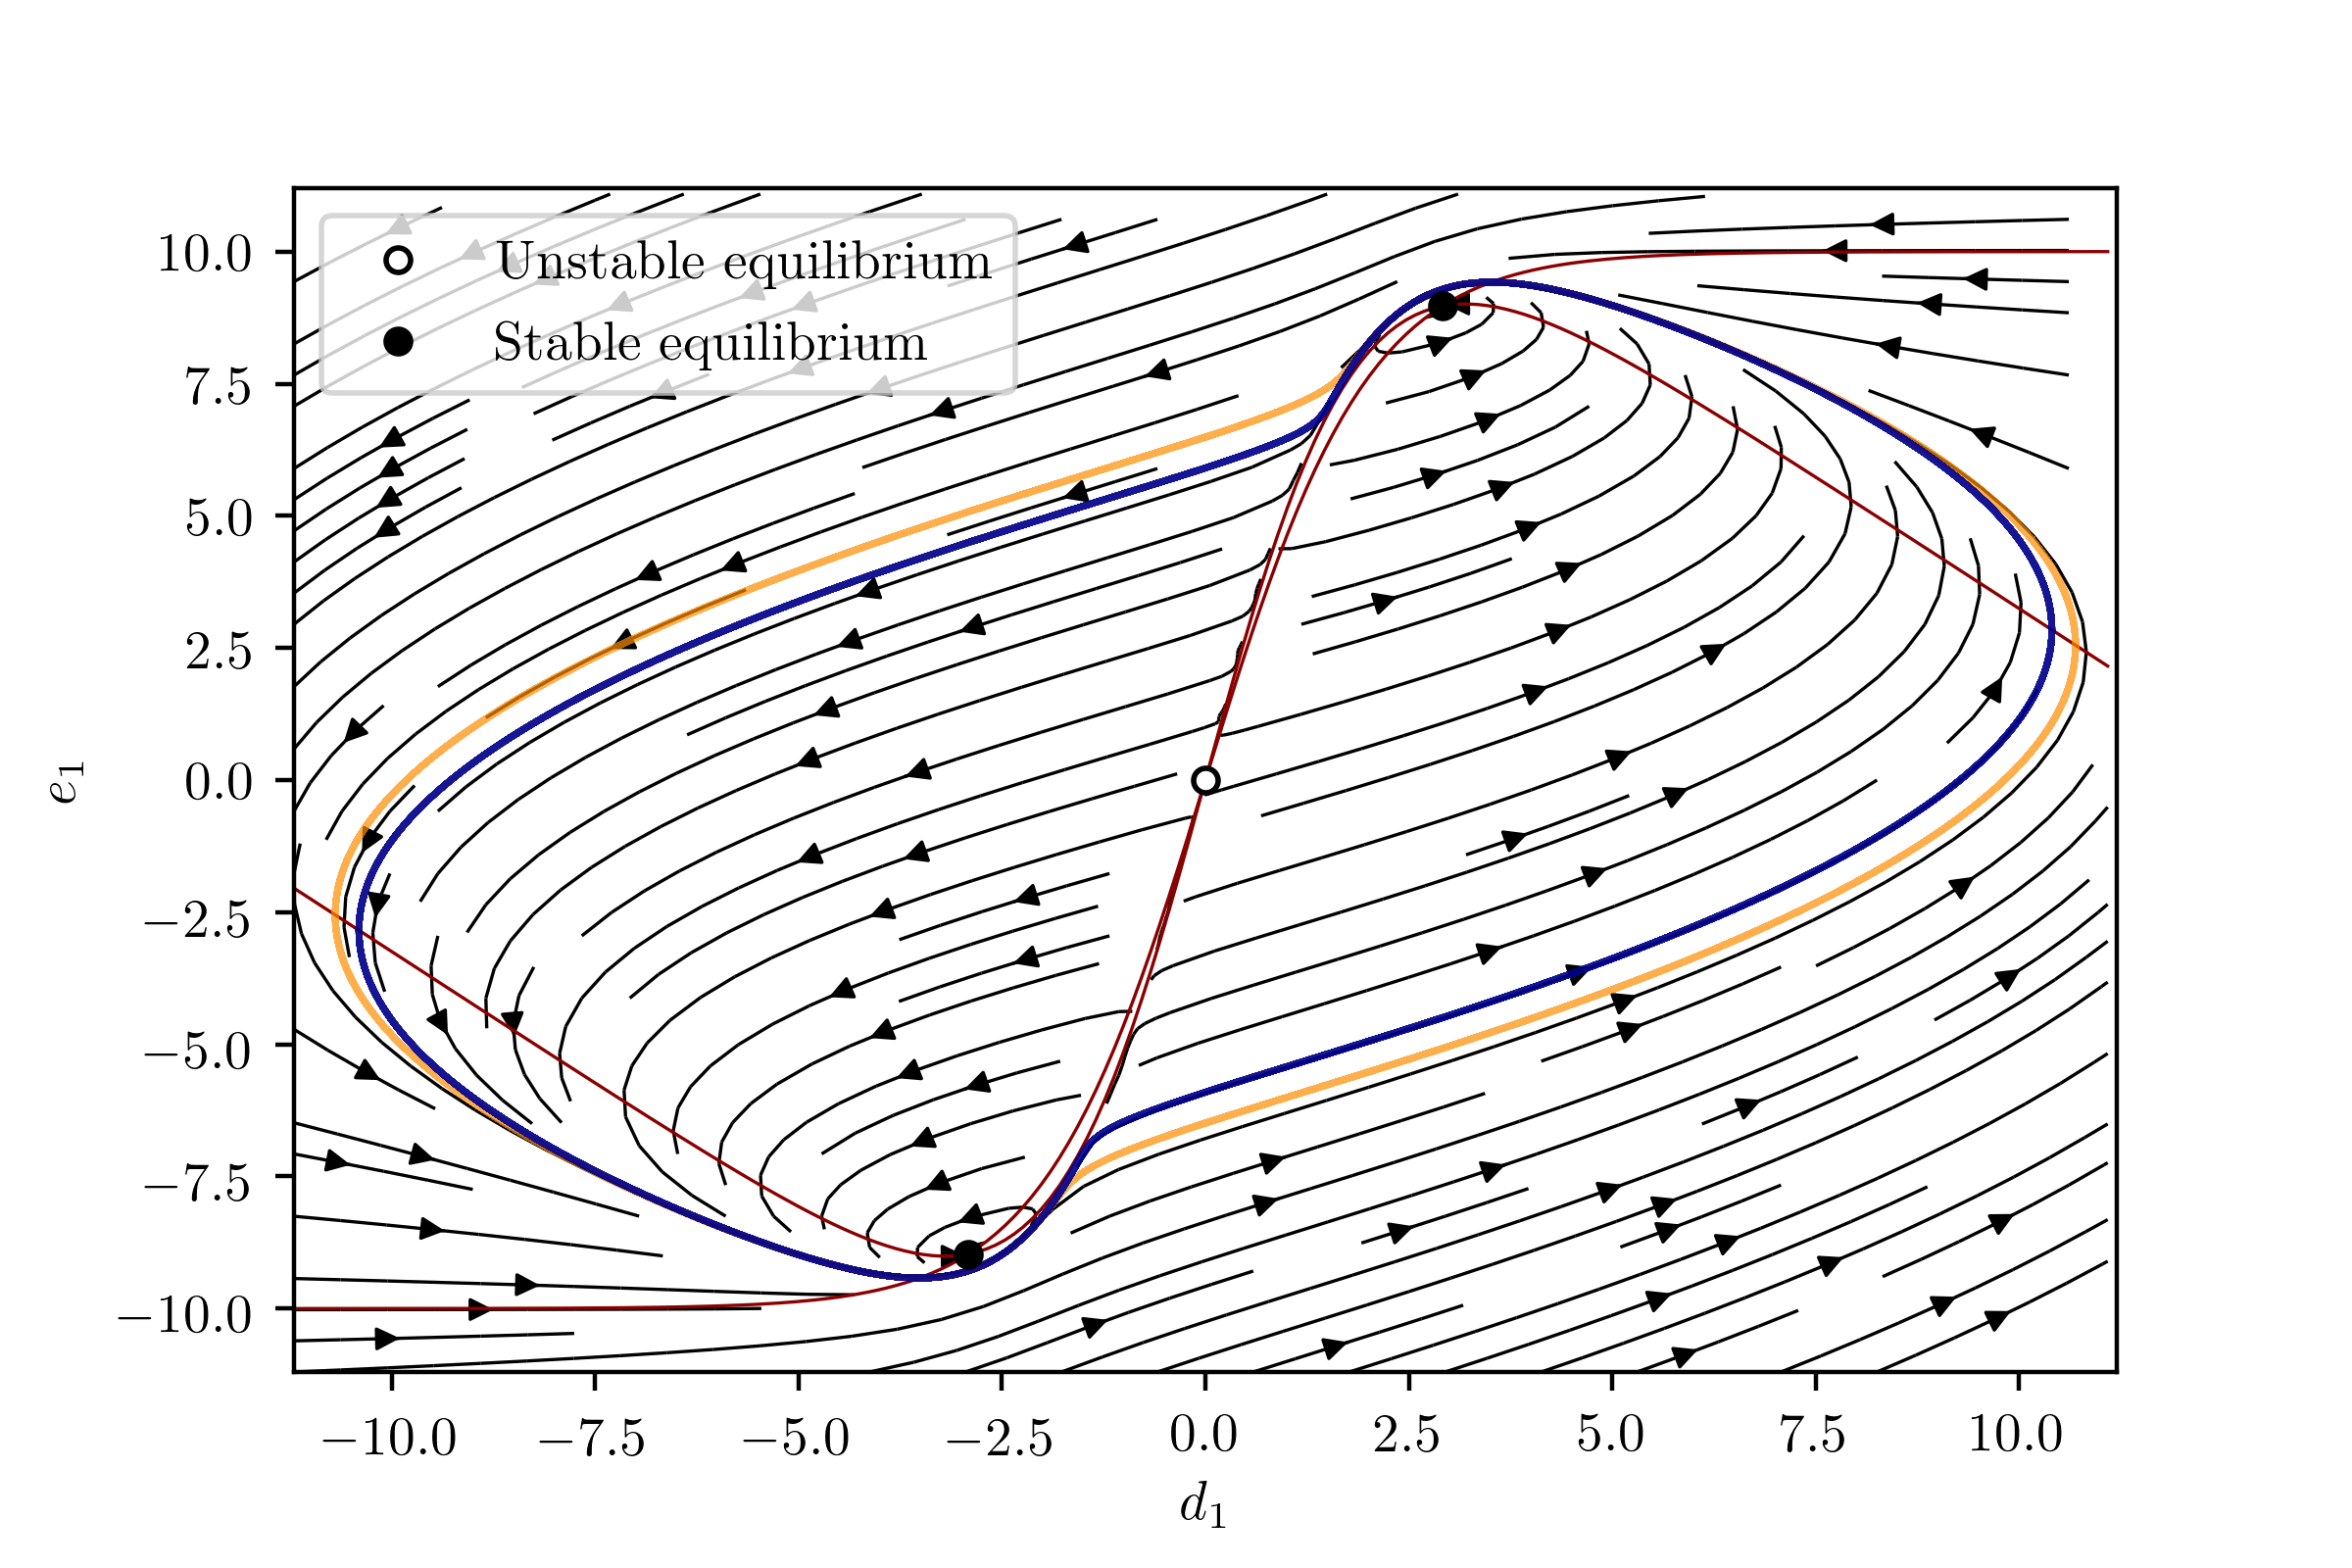
\includegraphics[width=\textwidth]{text/analysis/fig/2by2adapt/streamline_before_collapse.png}}
        \caption{\label{fig:eq2D_cycle_before_collapse} Phase portrait of system in \eqref{eq:diff_dynamics} for $k=13.24605,\ g_a=10,\ \tau_a=2$. The nullclines are shown in dark red; the streamline plot is shown in black; the outer stable limit cycle is shown in orange; the inner unstable limit cycle (obtained by backward integration in time) is shown in blue.}
\end{figure}


\begin{figure}[!h]
        \center{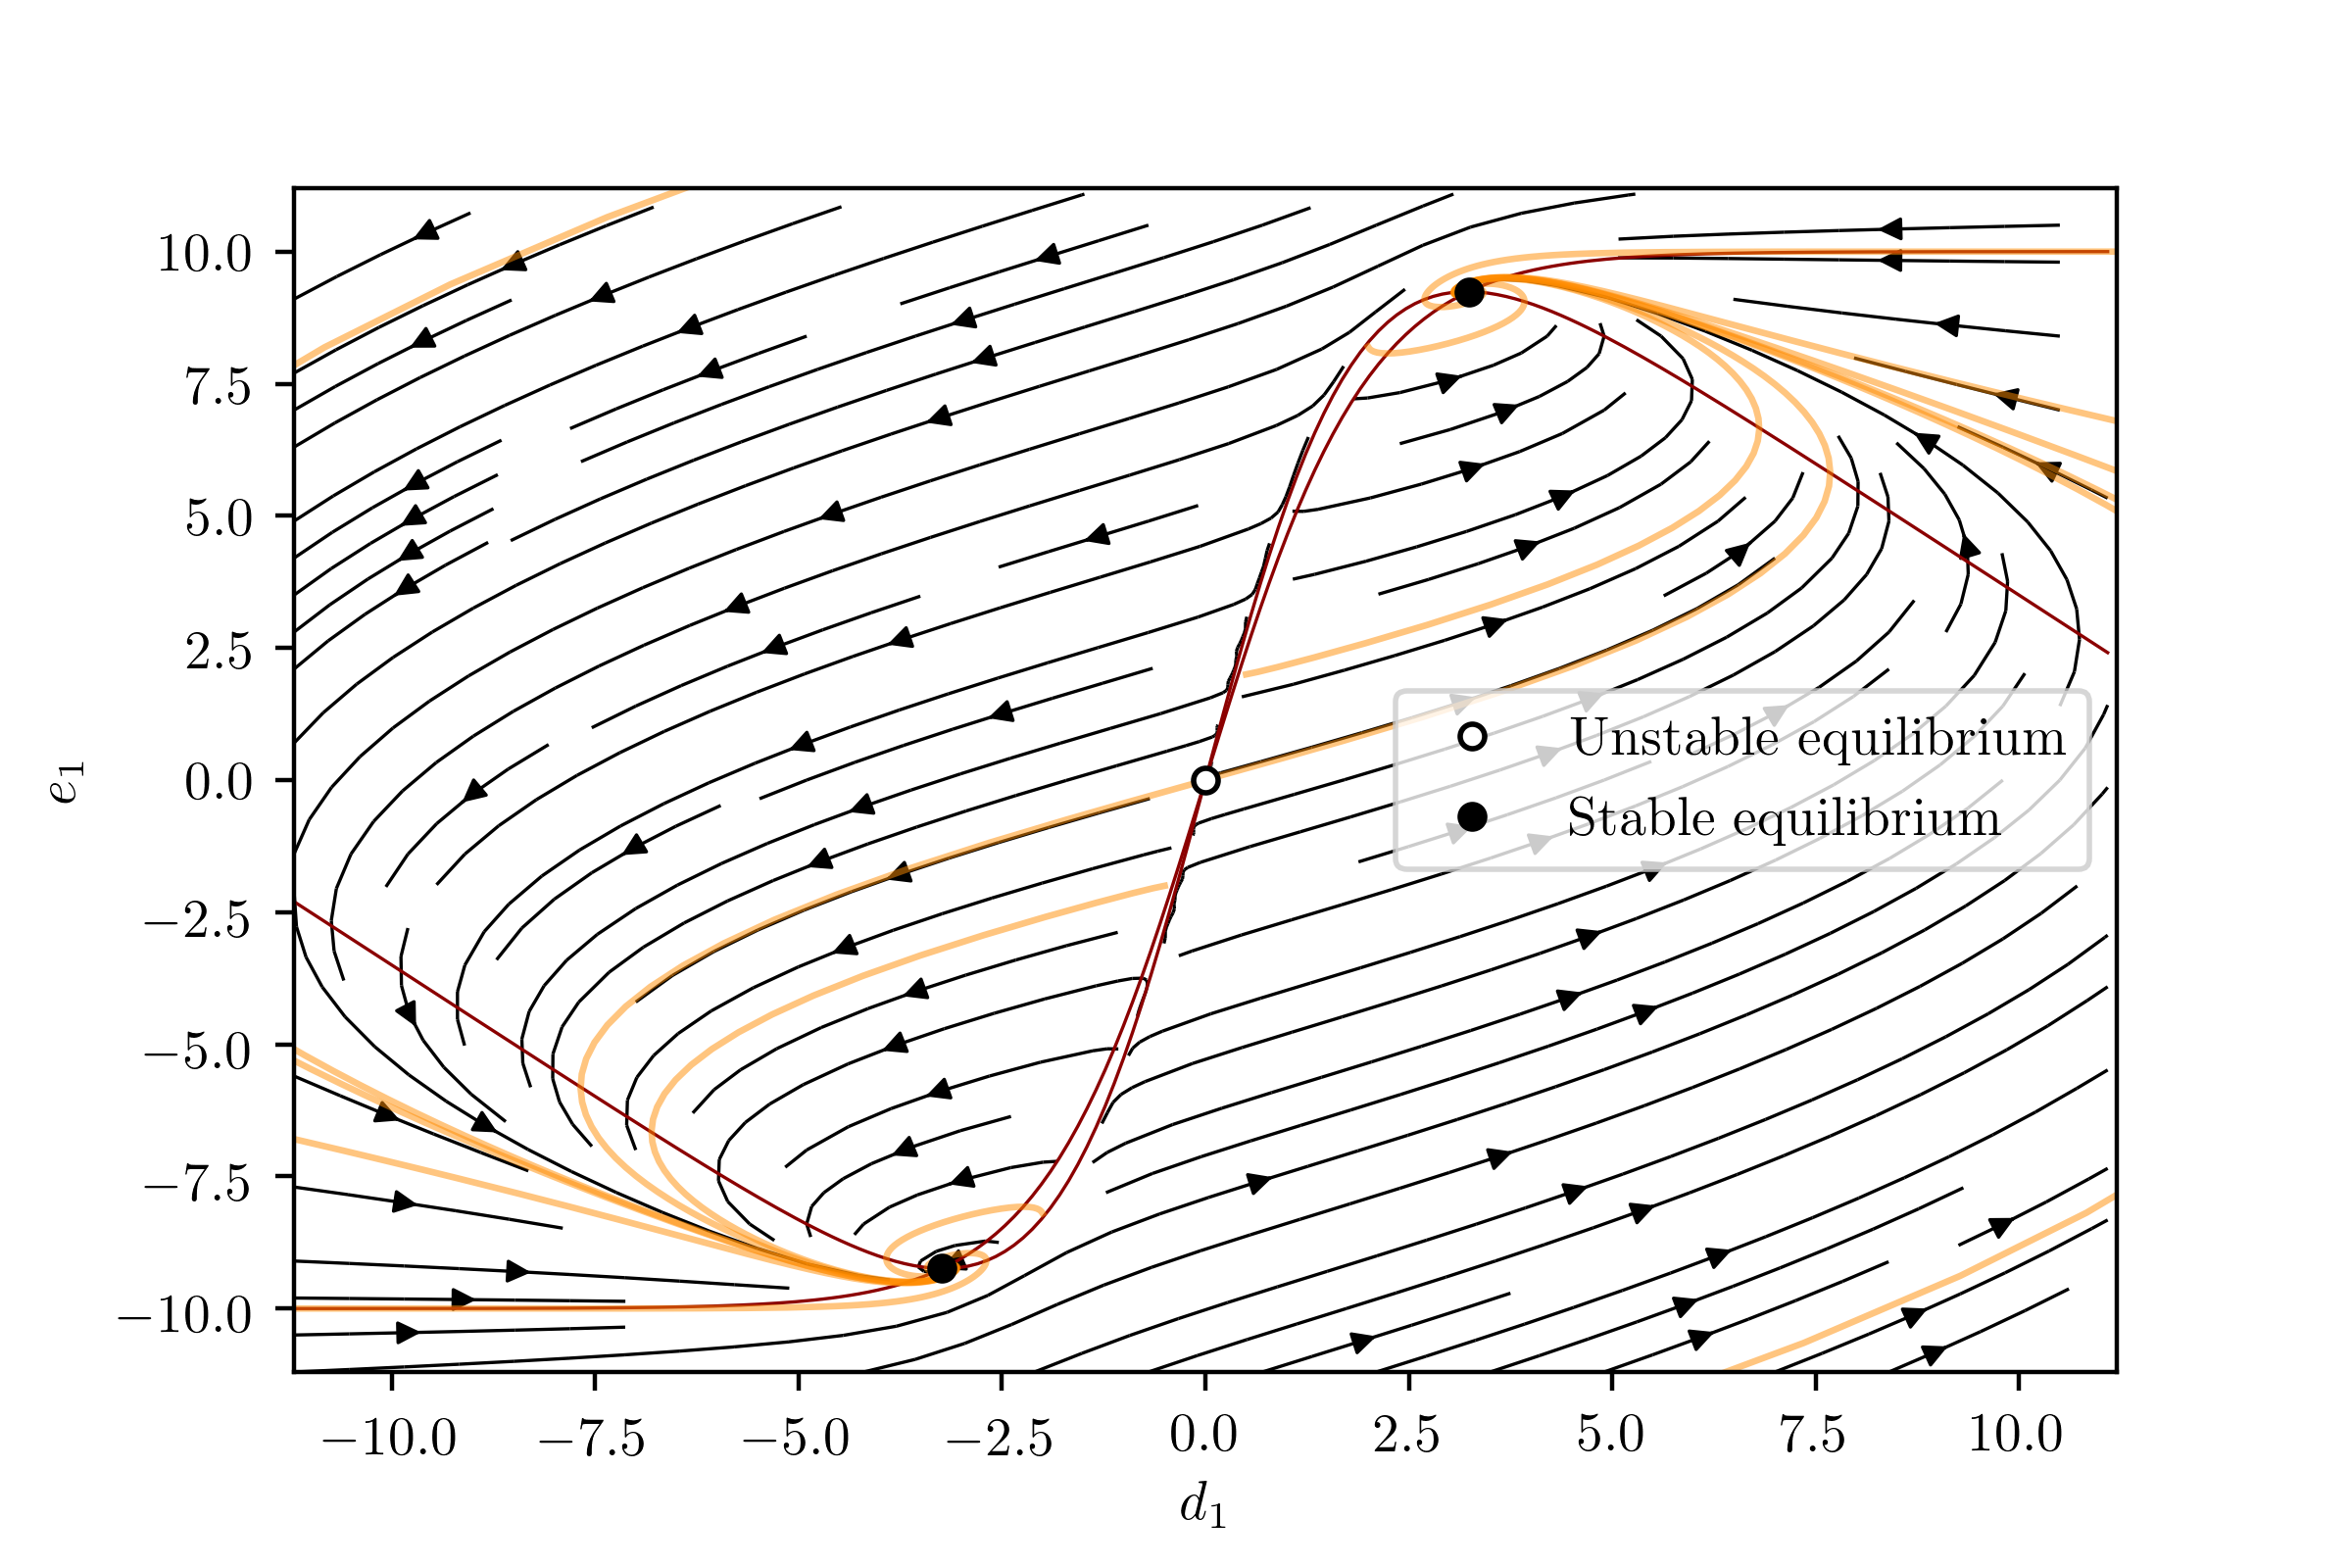
\includegraphics[width=\textwidth]{text/analysis/fig/2by2adapt/streamline_after_collapse.png}}
        \caption{\label{fig:eq2D_cycle_after_collapse} Phase portrait of system in \eqref{eq:diff_dynamics} for $k=13.5,\ g_a=10,\ \tau_a=2$. The nullclines are shown in dark red; the streamline plot is shown in black; several trajectories of the system with different initial conditions are shown in orange. }
\end{figure}

\paragraph{Bifurcation results discussion}
Even for a simple 4-dimensional oscillator, the dynamics of the system is quite rich and it qualitatively varies according to the variation of the parameter $k$.
The four most important situations above can be resumed as follows:
\begin{itemize}
    \item One globally stable equilibrium point with $k<2(1+\frac{1}{\tau_a})$ (\cref{fig:eq2D_focus})
    \item One globally stable limit cycle with $2(1+\frac{1}{\tau_a}) < k \lessapprox 12.69$ (\cref{fig:eq2D_cycle})
    \item One stable limit cycle and two stable equilibria with $12.69 \lessapprox k \lessapprox 13.24605$ (\cref{fig:adapt_zoom_tri_limt})
    \item Two stable equilibria with $k \gtrapprox 13.24605$ (\cref{fig:eq2D_cycle_after_collapse})
\end{itemize}

\iftrue
   \begin{figure*}[!h]
        \centering
        \begin{subfigure}[b]{1\textwidth}
            \centering
            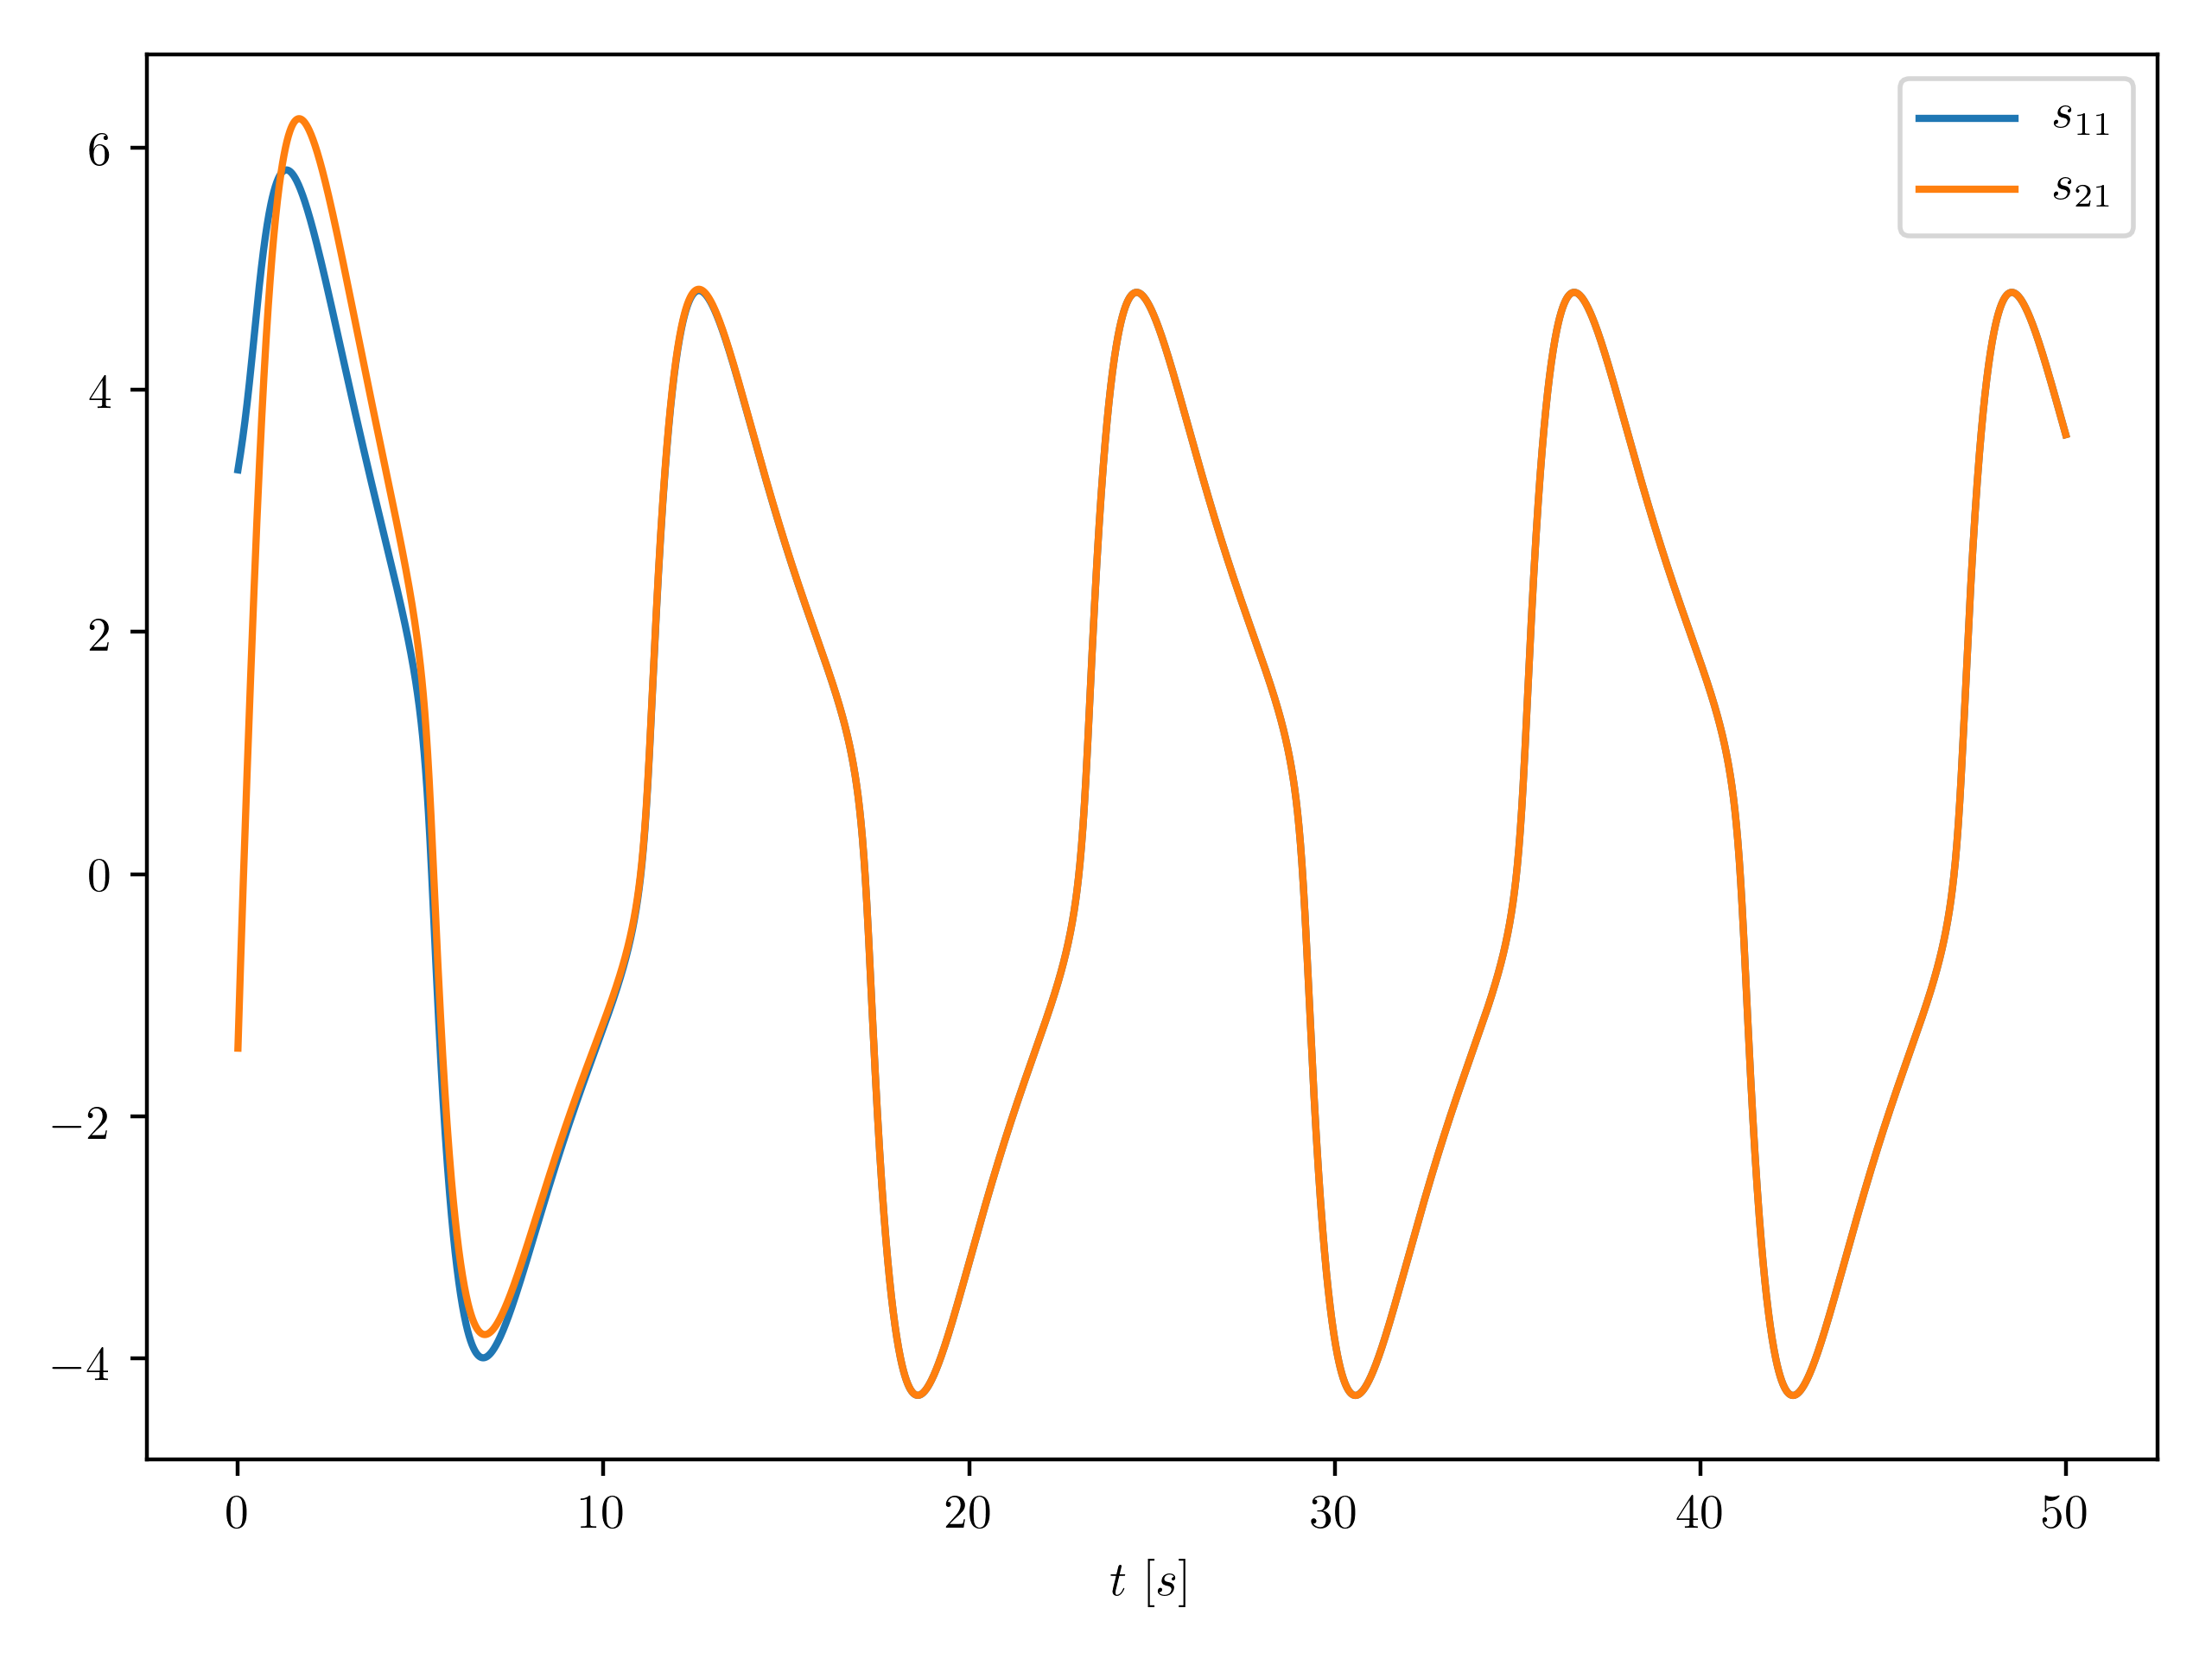
\includegraphics[width=\textwidth]{text/analysis/fig/2by2adapt/synch_2_mc_1.png}
        \end{subfigure}
        \vskip\baselineskip
        \begin{subfigure}[b]{1\textwidth}  
            \centering 
            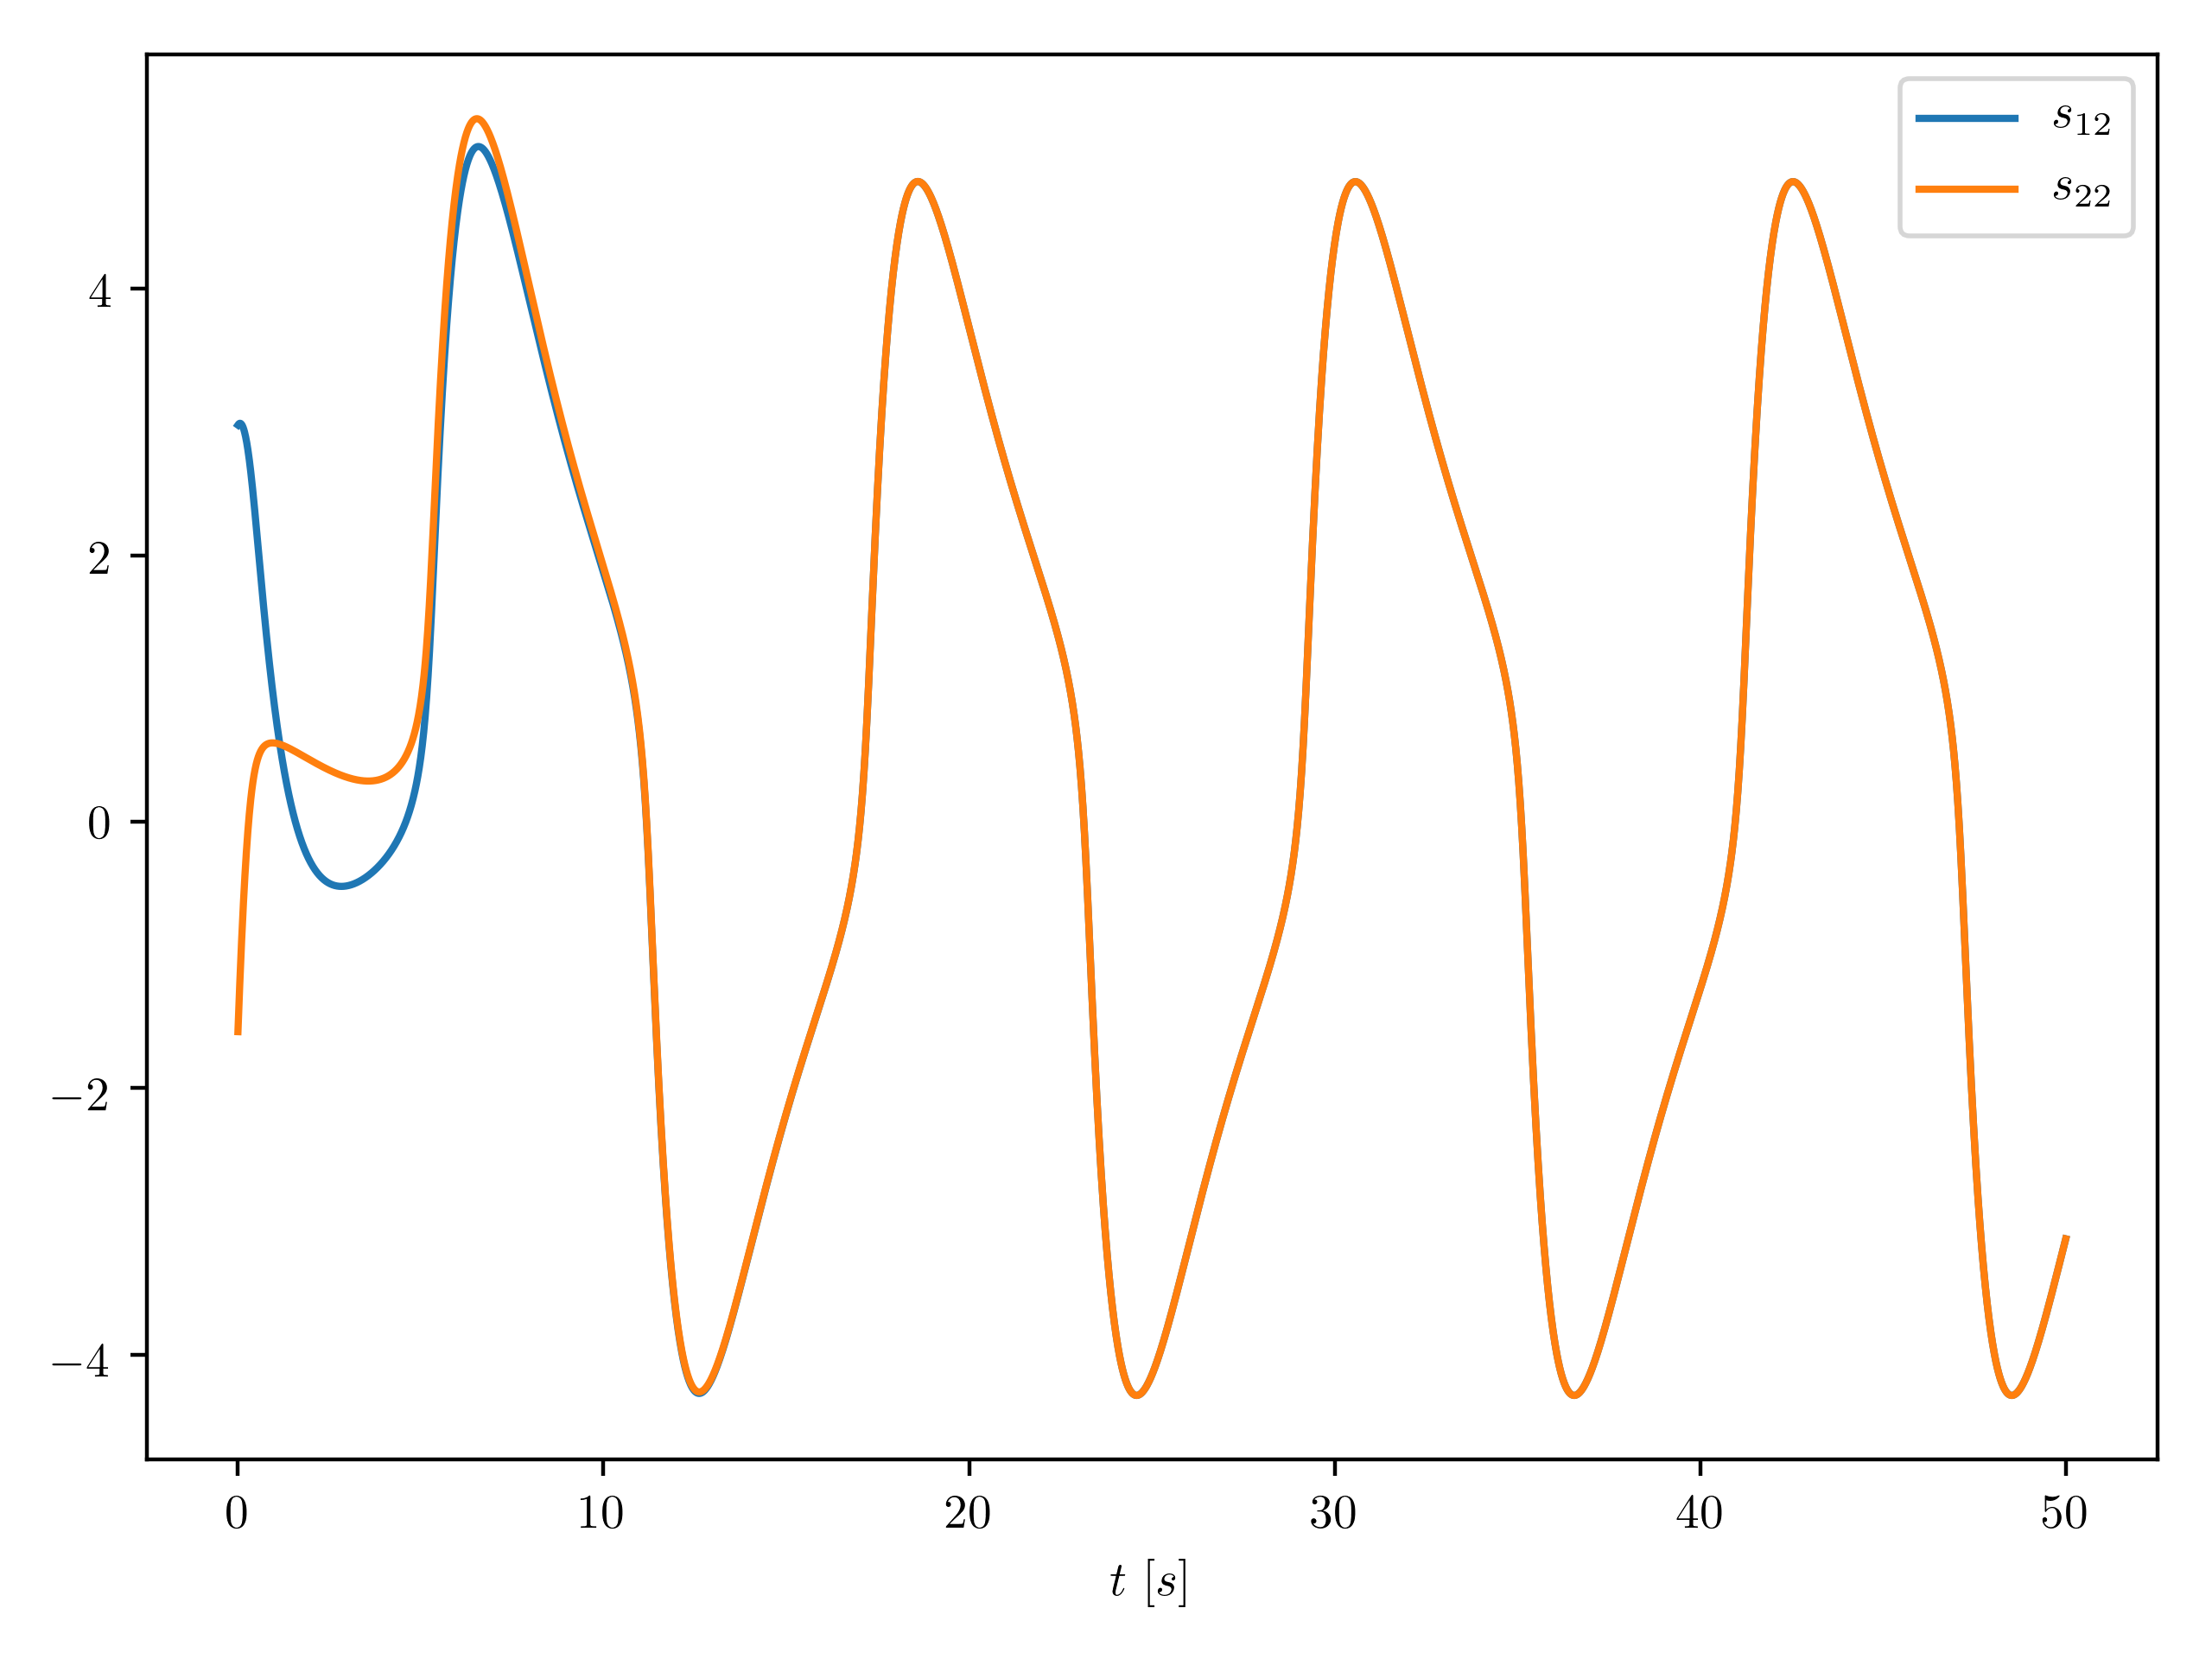
\includegraphics[width=\textwidth]{text/analysis/fig/2by2adapt/synch_2_mc_2.png}
        \end{subfigure}
        \caption{Phase portrait of system in \eqref{eq:diff_dynamics} for $k=13.15,\ g_a=10,\ \tau_a=2$. The nullclines are shown in dark red; the streamline plot is shown in black; the outer stable limit cycle is shown in orange; the inner unstable limit cycles (obtained by backward integration in time) are shown in blue. The two pictures show respectively the overall phase portrait (upper) and a zoom on the unstable limit cycle (lower).} 
        \label{fig:2D_limit_cycle}
    \end{figure*}
\fi